\documentclass[11pt, dvipdfmx]{beamer}
%\documentclass[8,9,10,11,12,14,17,20pt, dvips, handout]{beamer}
%%%%%%%%%%%  package  %%%%%%%%%%%
\usepackage{amssymb,amsmath,ascmac}
\usepackage{atbegshi}

\AtBeginShipoutFirst{\special{pdf:tounicode 90ms-RKSJ-UCS2}}
\usepackage{minijs}
\renewcommand{\kanjifamilydefault}{\gtdefault}
\usepackage{multirow}
\usepackage{bm}

\usepackage{tikz}
\usepackage{xparse}
\usetikzlibrary{shapes,arrows}
%% define fancy arrow. \tikzfancyarrow[<option>]{<text>}. ex: \tikzfancyarrow[fill=red!5]{hoge}
  \tikzset{arrowstyle/.style n args={2}{inner ysep=0.1ex, inner xsep=0.5em, minimum height=2em, draw=#2, fill=black!20, font=\sffamily\bfseries, single arrow, single arrow head extend=0.4em, #1,}}
  \NewDocumentCommand{\tikzfancyarrow}{O{fill=black!20} O{none}  m}{
    \tikz[baseline=-0.5ex]\node [arrowstyle={#1}{#2}] {#3 \mathstrut};}

%微分関連のマクロ
%
\newcommand{\diff}{\mathrm d}
\newcommand{\difd}[2]{\dfrac{\diff #1}{\diff #2}}
\newcommand{\difp}[2]{\dfrac{\partial #1}{\partial #2}}
\newcommand{\difdd}[2]{\dfrac{\diff^2 #1}{\diff #2^2}}
\newcommand{\difpp}[2]{\dfrac{\partial^2 #1}{\partial #2^2}}

\renewcommand\appendixname{Appendix}

%%%%%%%%%%%  theme  %%%%%%%%%%%

%%%%%
% Simple
%%%%%
%\usetheme{default}
%\usetheme{Pittsburgh}
%\usetheme{Rochester}
%\usetheme{Szeged}

%%%%%
% So So
%%%%%
%\usetheme{Singapore}
%\usetheme{CambridgeUS}
\usetheme{Copenhagen}
%\usetheme{Luebeck}
%\usetheme{Malmoe}
%\usetheme{Warsaw}

%%%%%
% No Heasder
%%%%%
%\usetheme{Madrid}
%\usetheme{Boadilla}

%%%%%
% No Footer
%%%%%
%\usetheme{Darmstadt}
%\usetheme{JuanLesPins}
%\usetheme{Montpellier}

%%%%%
% Color
%%%%%
%\usetheme{AnnArbor}

%%%%%
% Too much
%%%%%
%\usetheme{Berlin}
%\usetheme{Ilmenau}

%%%%%
% Right hand Side
%%%%%
%\usetheme{Goettingen}
%\usetheme{Marburg}

%%%%%
% Left hand Side
%%%%%
%\usetheme{PaloAlto}


%%%%%%%%%%%  inner theme  %%%%%%%%%%%
\useinnertheme{default}
%\useinnertheme{circles}
%\useinnertheme{inmargin}
%\useinnertheme{rectangles}
%\useinnertheme{rounded}


%%%%%%%%%%%  outer theme  %%%%%%%%%%%
\useoutertheme{default}
%\useoutertheme{miniframes}
%\useoutertheme{infolines}
%\useoutertheme{miniframes}
%\useoutertheme{smoothbars}
%\useoutertheme{sidebars}
%\useoutertheme{split}
%\useoutertheme{shadow}
%\useoutertheme{tree}
%\useoutertheme{smoothtree}


%%%%%%%%%%%  color theme  %%%%%%%%%%%
%\usecolortheme{structure}
%\usecolortheme{sidebartab}
%\usecolortheme{albatross}
%\usecolortheme{beetle}
%\usecolortheme{dove}
%\usecolortheme{crane}
%\usecolortheme{fly}
%\usecolortheme{seagull}
%\usecolortheme{wolverine}
%\usecolortheme{beaver}
%\usecolortheme{lily}
%\usecolortheme{orchid}
%\usecolortheme{rose}
%\usecolortheme{whale}
%\usecolortheme{seahorse}
%\usecolortheme{dolphin}


%%%%%%%%%%%  font theme  %%%%%%%%%%%
\usefonttheme{professionalfonts}
%\usefonttheme{default}
%\usefonttheme{serif}
%\usefonttheme{structurebold}
%\usefonttheme{structureserif}
%\usefonttheme{structuresmallcapsserif}


%%%%%%%%%%%  degree of transparency  %%%%%%%%%%%
%\setbeamercovered{transparent=30}

%\setbeamercolor{item}{fg=red}
\setbeamertemplate{items}[default]

%%%%%%%%%%%  numbering  %%%%%%%%%%%
%\setbeamertemplate{numbered}

\setbeamertemplate{navigation symbols}{}
%%%%%%%%%%%%%%%%%%%%%%%%%%%%%%%%%%%
\title
[MD シミュレーションによるネットワークポリマーのゴム弾性]
{MD シミュレーションによる\\ネットワークポリマーのゴム弾性}
\author[東亞合成 佐々木、大村]{佐々木裕}
\institute[東亞合成]{東亞合成}
\date{December 19, 2018}
%%%%%%%%%%%%%%%%%%%%%%%%%%%%%%%%%%
\begin{document}
%%%%%%%%%%%%%%%%%%%%%%%%%%%%%%%%%%
\begin{frame}\frametitle{}
	\titlepage
\end{frame}
%%%%%%%%%%%%%%%%%%%%%
\section{はじめに}
%%%%%%%%%%%%%%%%%
\begin{frame}
\LARGE{はじめに}
\end{frame}
%%%%%%%%%%%%%%%%%%%%%%%%%%%%
\subsection{高分子材料と耐久性}
%%%%%%%%%%%%%%%%%%%%%%%%%%%%
\begin{frame}
\frametitle{高分子材料への期待と不安}
地球温暖化対策の CO$_2$ 削減への一つの主要なアイテムとして、\\
{\Large
{\color{red}「自動車を中心とした運送機器の抜本的な軽量化」}
}\\
が提唱されている。
\begin{block}{高分子材料への期待}
	\begin{itemize}
	\item
	現行の鉄鋼主体$ \Rightarrow$ 高分子材料を含むマルチマテリアル化
	
	\item
	高分子材料によるマルチマテリアル化のポイント
		\begin{itemize}
		\item
		高い比強度の有効利用
		\item
		特徴を生かした適材適所 $\Leftrightarrow$ 適切な接合方法の選択
			\Large
			\begin{itemize}
			\item
			{\color{red} 「接着接合」への高分子の利用}
			\item
			{\color{red} 「柔らかさを生かした弾性接着接合」への期待}
			\end{itemize}
		\item
		{\color{blue}耐久性が不明確(特に疲労破壊に対して)}
		\end{itemize}
	\end{itemize}
\end{block}
\end{frame}
%%%%%%%%%%%%%%%%%%%%%%%%%%%%
\begin{frame}
\frametitle{マルチスケールと物性}
\href{http://j-parc.jp/ja/topics/2015/Pulse151112.html}{J-PARCの広報サイト}から引用。
\small
『SPring-8・J-PARC・スーパーコンピュータ「京」を連携活用させたタイヤ用新材料開発技術「ADVANCED 4D NANO DESIGN」を確立』
\centering
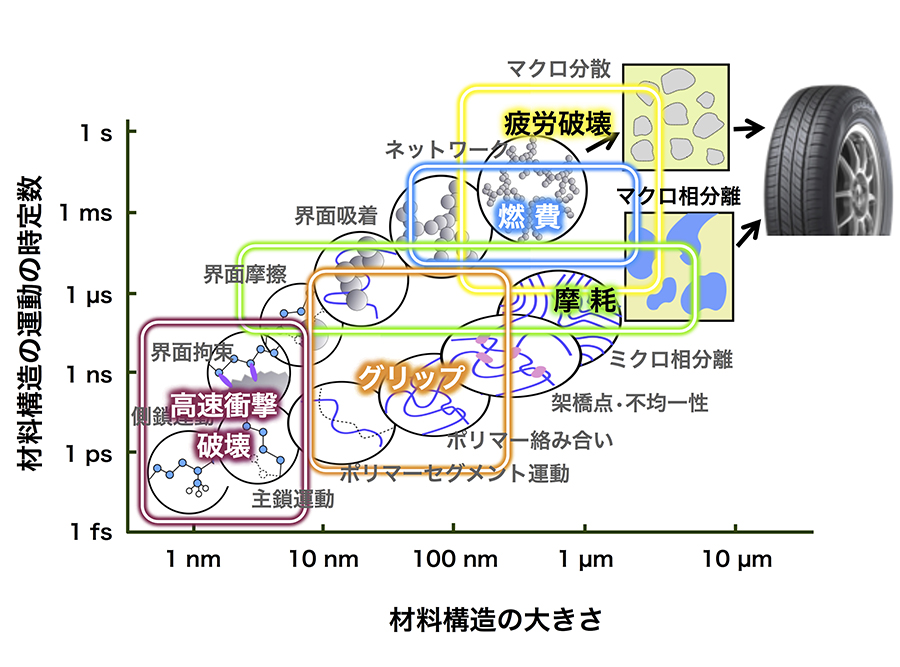
\includegraphics[width=75mm]{./fig/press151112_02.jpg}
\end{frame}
%%%%%%%%%%%%%%%%%%%%%%%%%%%%
\begin{frame}
\frametitle{スケールと特徴的構造}
\href{http://j-parc.jp/ja/topics/2015/Pulse151112.html}{J-PARCの広報サイト}から引用。
\small
『SPring-8・J-PARC・スーパーコンピュータ「京」を連携活用させたタイヤ用新材料開発技術「ADVANCED 4D NANO DESIGN」を確立』
\centering
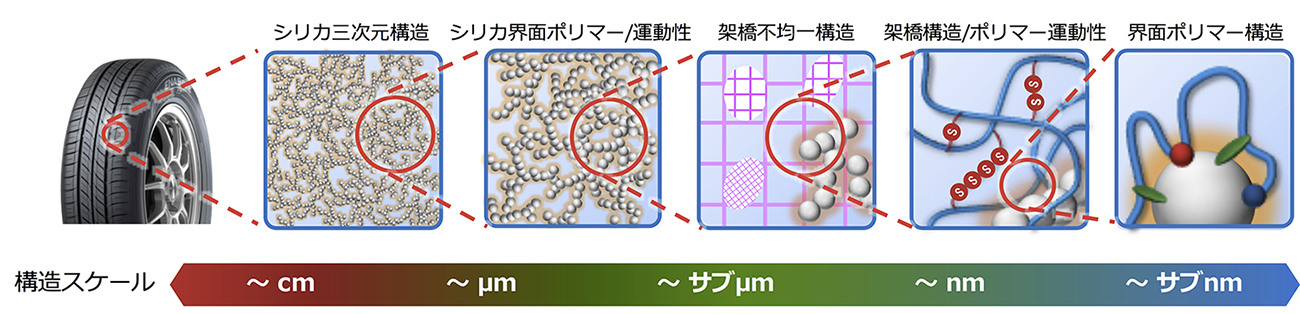
\includegraphics[width=105mm]{./fig/press151112_03.jpg}
\end{frame}
%%%%%%%%%%%%%%%%%%%%%%%%%%%%
\subsubsection{破壊工学とエネルギー散逸}
%%%%%%%%%%%%%%%%%%%%%%%%%%%%%%
\begin{frame}
\frametitle{破壊工学とエネルギー散逸}
\begin{columns}[totalwidth=1\textwidth]
\column{.48\textwidth}
\vspace{-2mm}
\begin{exampleblock}{破壊工学の考え方}
\small
\begin{itemize}
\item
「クラック近傍での応力集中を如何に抑制するか」
\item 
クラック先端での\alert{局所降伏}
\end{itemize}
\end{exampleblock}
\centering
	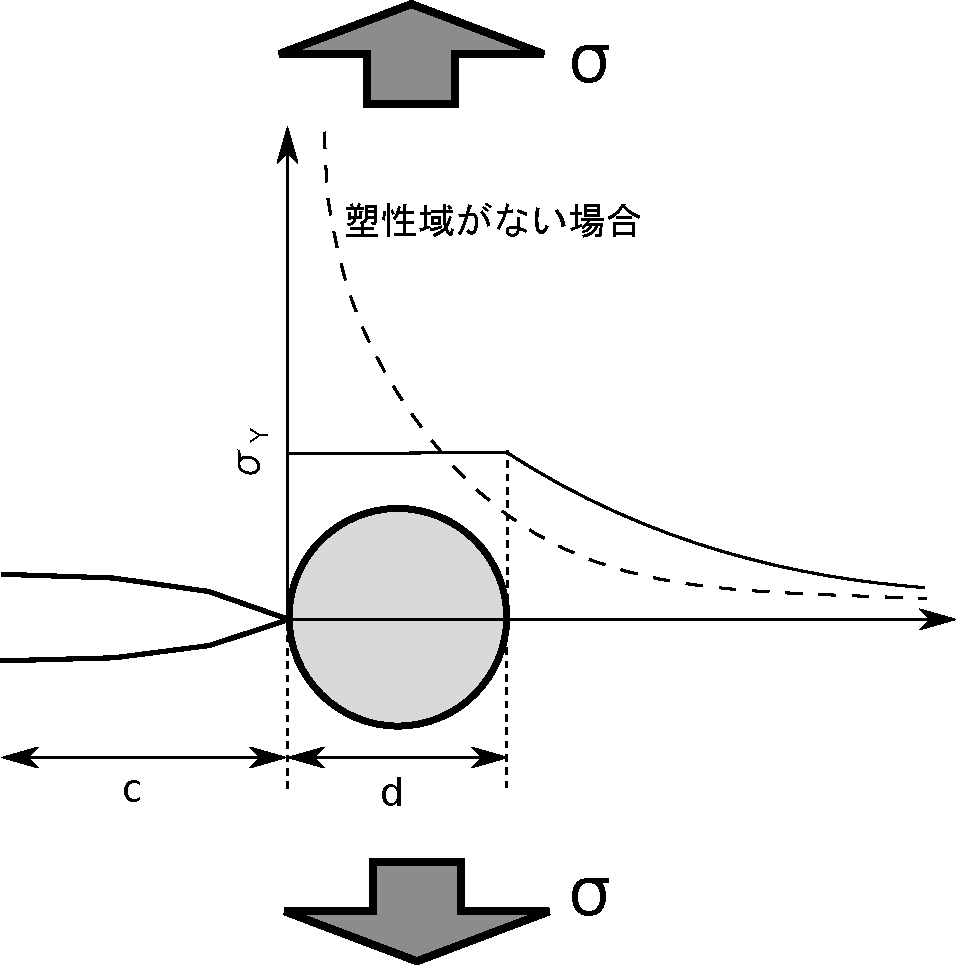
\includegraphics[width=40mm]{./fig/Crack_Yield.pdf}
\column{.48\textwidth}
\begin{alertblock}{Andrews 理論}
\small
	\begin{itemize}
	\item
	クラック先端で\alert{ヒステリシス由来のエネルギー散逸}
	\item
	ひずみエネルギー開放率低減
	\end{itemize}
\end{alertblock}
\centering
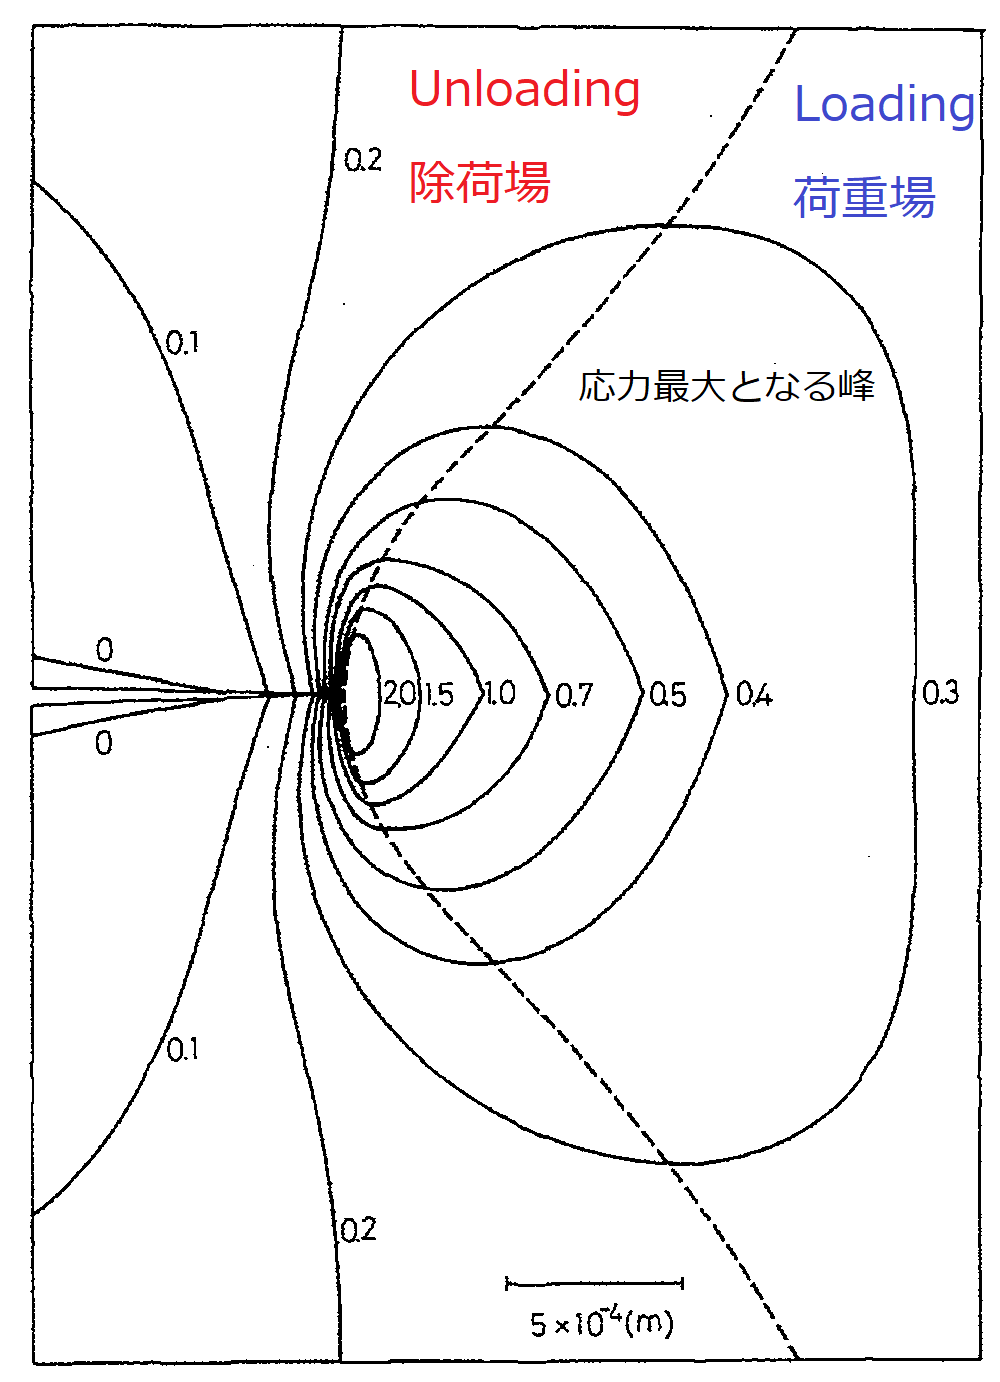
\includegraphics[width=30mm]{./fig/crack.png}	
\end{columns}
\end{frame}
%%%%%%%%%%%%%%%%%%%%%%%%%%%
\begin{frame}
\frametitle{本研究の目標とアプローチ}
\vspace{-2mm}
\begin{exampleblock}{本研究の目標とアプローチ}
\begin{itemize}
\item
目標\\
破壊耐性に優れた軽量材料の創成とその設計指針の明確化
\item
アプローチ
	\begin{itemize}
	\item
	可逆性に優れた材料としてゴム材料を選択。
	\item
	構造明確なネットワークの構築のために超分子ネットワーク。
	\item
	既知のモデルとの\color{red}多数の整合点と、興味深い不整合\color{black}を確認。
	\item
	\color{red}シミュレーションでマルチスケールモデル\color{black}を構築したい。
	\end{itemize}
\end{itemize}
\end{exampleblock}
\vspace{-2mm}
\begin{alertblock}{シミュレーションでやりたいこと}
\begin{itemize}
\item
できるだけ\alert{単純化したモデルで小さなスケール}から始めたい。
\item
まずは、長さの揃ったストランドで MD シミュレーション
\item
最終的に、亀裂先端の挙動を FEM シミュレーション
\end{itemize}
\centering
{\color{red}\Large「オッカムの剃刀」}
\end{alertblock}
\end{frame}
%%%%%%%%%%%%%%%%%%%%%%%%%%%%%%%%%%%%%%%%%%%%%
\subsection{規則ネットワーク構造での検討結果}
%%%%%%%%%%%%%%%%%%%%%%%%%%%
\begin{frame}
\frametitle{これまでのMDシミュレーション}
\begin{columns}[totalwidth=1\textwidth]
\column{.49\textwidth}
ストランド長を一定とした\\規則構造
\begin{itemize}
 \item 
 分岐数 
 	\begin{itemize}
 	\item  
 	三分岐\\
 	K4 構造
 	\item
 	四分岐\\
 	ダイヤモンド構造
	\end{itemize}
 \item 
 ストランド
 	\begin{itemize}
 	\item  
 	KG鎖\\
 	LJ ポテンシャルにより、排除体積効果を導入
 	\item
	素抜け鎖\\
	長距離相互作用を無視した理想鎖
	\end{itemize}
\end{itemize}
\column{.49\textwidth}
K4 構造
\vspace{-3mm}
\begin{figure}
\centering
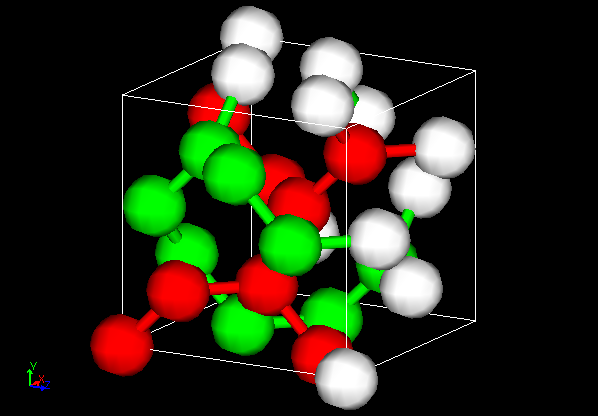
\includegraphics[width=0.7\textwidth]{./fig/K4_d.png}
\end{figure}
ダイヤモンド構造
\vspace{-3mm}
\begin{figure}
\centering
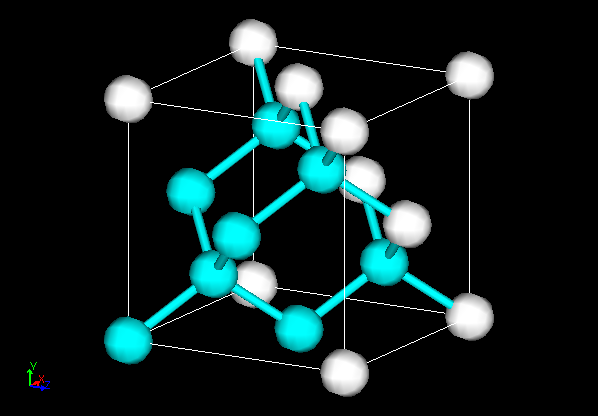
\includegraphics[width=0.7\textwidth]{./fig/dia.png}
\end{figure}
\end{columns}
\end{frame}
%%%%%%%%%%%%%%%%%%%%%%%%%%%%%%%%%%%%%%
\begin{frame}
\frametitle{規則ネットワーク構造での検討結果}

\vspace{-2mm}
\small
\begin{alertblock}{規則ネットワーク構造の振る舞い}
\begin{itemize}
\item
一軸伸長結果
	\begin{itemize}
	\item
	\alert{アフィンネットワークモデルの挙動}を示した\\\alert{分岐数、ストランドの性質によらず}(KGでも素抜けでも)
	\item
	伸びきり効果をほぼ再現
	\end{itemize}
\item
応力緩和挙動から主緩和が\alert{ラウスモードの最長緩和時間程度}と確認
\item
主緩和の近傍で大きな\alert{力学的ヒステリシス}がみられた
\end{itemize}
\end{alertblock}
\begin{columns}[totalwidth=1\textwidth]
\column{.3\textwidth}
\scriptsize
一軸伸長結果
\vspace{-5mm}
\begin{figure}
\centering
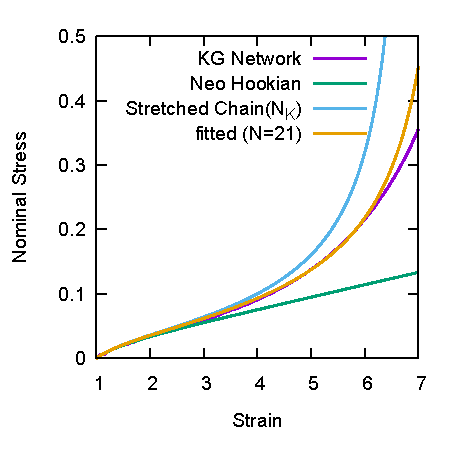
\includegraphics[width=0.9\textwidth]{./fig/SS_Kuhn.pdf}
\end{figure}
\column{.3\textwidth}
\scriptsize
応力緩和挙動
\vspace{-5mm}
\begin{figure}
\centering
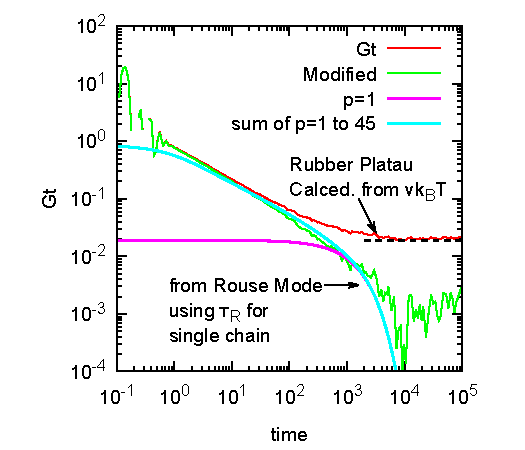
\includegraphics[width=0.9\textwidth]{./fig/Gt_loglog.pdf}
\end{figure}
\column{.3\textwidth}
\scriptsize
力学的ヒステリシス
\vspace{-5mm}
\begin{figure}
\centering
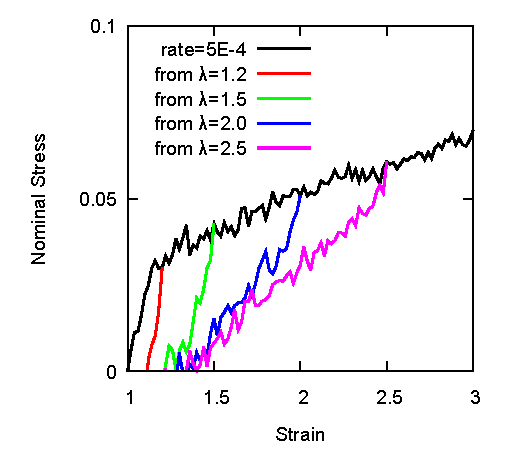
\includegraphics[width=0.9\textwidth]{./fig/N44_rev_SS.pdf}
\end{figure}
\end{columns}
\end{frame}
%%%%%%%%%%%%%%%%%%%%%%
\subsection{本発表の内容}
%%%%%%%%%%%%%%%%%%%%%%
\begin{frame}
\frametitle{本発表の内容}
\vspace{-2mm}
\begin{exampleblock}{本研究の目標とアプローチ}
\begin{itemize}
\item
目標\\
破壊耐性に優れた軽量材料の創成とその設計指針の明確化
\item
アプローチ
	\begin{itemize}
	\item
	可逆性に優れた材料としてゴム材料を選択。
	\item
	構造明確なネットワークの構築のために超分子ネットワーク。
	\item
	既知のモデルとの\color{red}多数の整合点と、興味深い不整合\color{black}を確認。
	\item
	\color{red}シミュレーションでマルチスケールモデル\color{black}を構築したい。
	\end{itemize}
\end{itemize}
\end{exampleblock}
\vspace{-1mm}
\begin{alertblock}{出来ていないこと}
ファントムネットワーク構造の挙動の明確化。
\end{alertblock}
\vspace{-1mm}
\begin{block}{本発表の内容}
本発表では、ネットワーク構造にランダム性を導入することで、ファントムネットワークモデルの構築を検討した。
\end{block}
\end{frame}
%%%%%%%%%%%%%%%%%%%%%%%%%%
\section{検討内容}
%%%%%%%%%%%%%%%%%%%%%%%%%%
%%%%%%%%%%%%%%%%%
\begin{frame}
\LARGE{検討内容}
\end{frame}
%%%%%%%%%%%%%%%%%%%%%%%%%%%%%%%%%
\subsection{ランダムネットワーク構造の作成}
%%%%%%%%%%%%%%%%%%%%%%%%%%
\begin{frame}
\frametitle{ランダムなネットワークの作成}
\small
\vspace{-2mm}
\begin{block}{ここでのランダムの定義}
\begin{itemize}
\item
ユニットセルの連なりとしてネットワークを考え、
\item
各ユニットセルごとにその内部の接続性をランダムとする。
\item
これは、\alert{各ノードの隣接関係をランダム}にすることに対応。
\end{itemize}
\end{block}
\vspace{-2mm}
\begin{exampleblock}{アルゴリズム}
\begin{enumerate}
\item
\alert{実空間}で8-Chain Model で初期構造を作成。\\(ストランド長:自由鎖の二乗平均末端間距離)
\item
初期構造のジオメトリーに対応した\alert{トポロジーモデル}を用いて、
	\begin{itemize}
 	\item 
 	ラプラシアン行列で\alert{全体の連結性を確認}しながら、
 	\item
 	\alert{ランダム}に選択した\alert{結合(エッジ)を除去}して、
 	\item
	8 分岐からノードごとのエッジ数(分岐数)に。
	\end{itemize}	
\item
トポロジーモデルに対応するように初期構造からストランド除去
\end{enumerate}
%\color{red} こうすれば、実空間で遠く離れたノードをつなげることはない。
\end{exampleblock}
\end{frame}
%%%%%%%%%%%%%%%%%%%%%%%%%%
\begin{frame}
\frametitle{変換例}
\begin{columns}[totalwidth=1\textwidth]
\column{.48\textwidth}
\begin{block}{実空間での初期構造}
\small
\begin{itemize}
\item
$2\times2\times2$ 個のユニットセル
\vspace{-2mm}
\begin{figure}
\centering
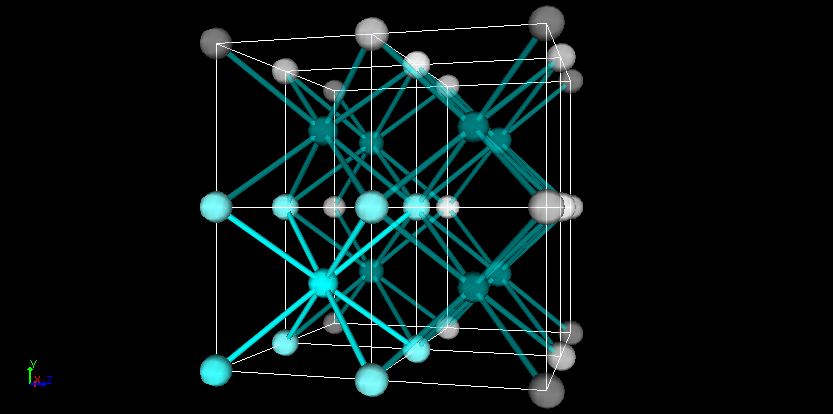
\includegraphics[width=0.8\columnwidth]{./fig/8_per.png}
\end{figure}
\vspace{-2mm}
\item
\vspace{-2mm}
ユニットセルから除去
\vspace{-2mm}
\begin{figure}
\centering
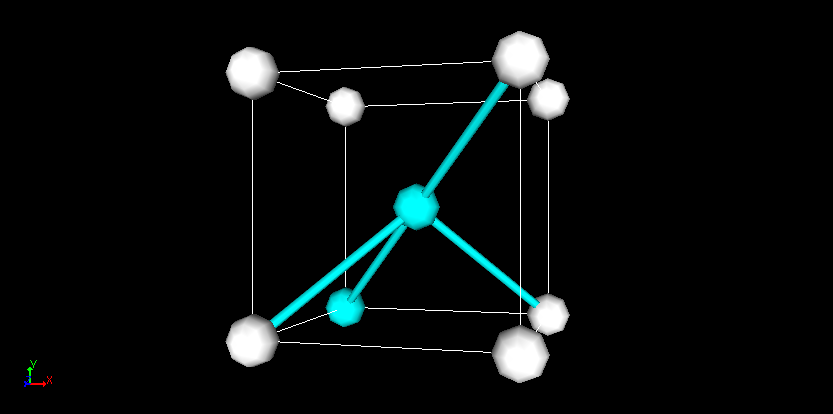
\includegraphics[width=0.8\columnwidth]{./fig/8_4.png}
\end{figure}
\end{itemize}
\end{block}
\column{.48\textwidth}
\begin{exampleblock}{トポロジーモデル}
\small
分岐数を4に減じたトポロジーモデル
\vspace{-2mm}
\begin{figure}
\centering
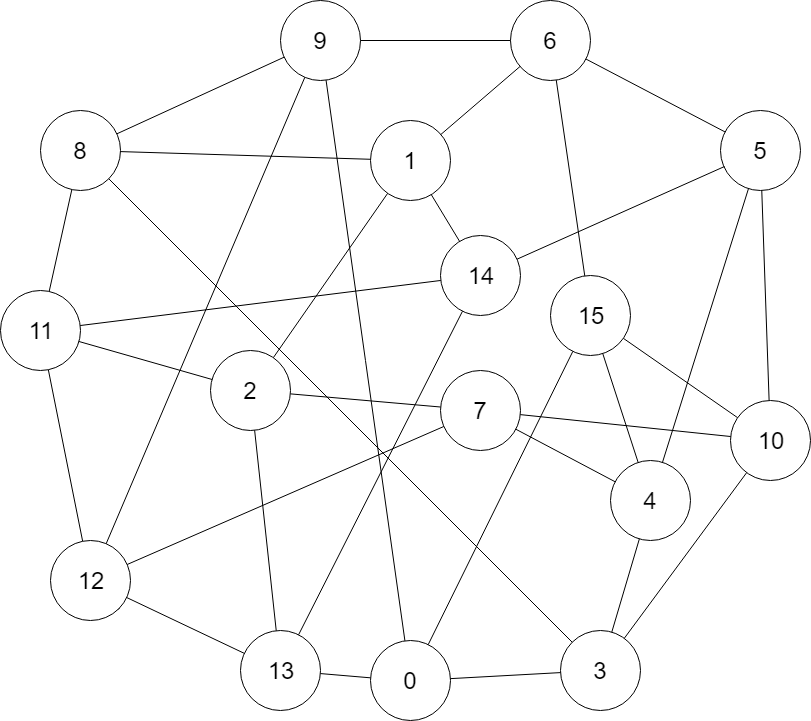
\includegraphics[width=\columnwidth]{./fig/Network.png}
\end{figure}
\end{exampleblock}
\end{columns}
\end{frame}
%%%%%%%%%%%%%%%%%%%
\subsection{シミュレーション結果(ストランドの末端間距離)}
%%%%%%%%%%%%%%%%%%%%%%%%%%%
\begin{frame}
\frametitle{シミュレーション結果(ストランドの末端間距離)}
\vspace{-3mm}
\begin{columns}[totalwidth=\linewidth]
\column{.48\linewidth}
\begin{block}{検討対象}
\begin{itemize}
\item
ストランド
	\begin{itemize}
	\item 
	素抜け鎖
 	\item 
 	ボンド:ハーモニック
 	\item
 	セグメント数 N=20 
	\end{itemize}
\item
ランダムネットワーク
	\begin{itemize}
	\item
	三分岐モデル($f=3$)
	\item
	システムサイズ\\
	$6\times 6\times 6$
	\end{itemize}
\end{itemize}
\end{block}
\column{.48\linewidth}
\begin{figure}
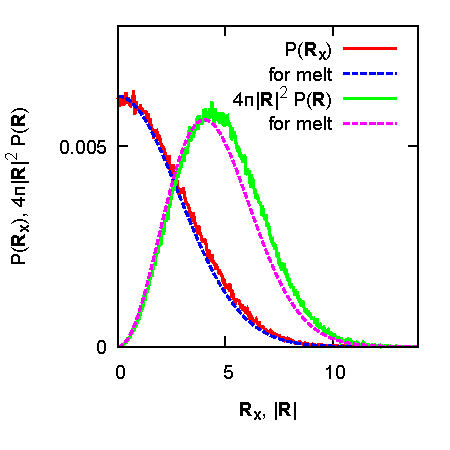
\includegraphics[width=\columnwidth]{./fig/PR.pdf}
\end{figure}
\end{columns}
\vspace{-2mm}
\begin{exampleblock}{ストランド長の分布関数}
\begin{itemize}
\item
ホモポリマーメルトの分布関数の形状をほぼ再現
\item
末端間距離が若干長い(平均で数 \% 程度)
\end{itemize}
\end{exampleblock}
\end{frame}
%%%%%%%%%%%%%%%%%%%
\subsection{シミュレーション結果(一軸伸長)}
%%%%%%%%%%%%%%%%%%%%%%%%%%
\begin{frame}
\frametitle{Phantom Network Model}
\begin{columns}[totalwidth=1\textwidth]
\column{.48\textwidth}
\begin{block}{壁面に末端が固定された効果}
\begin{itemize}
\item
壁面に末端が固定
	\begin{itemize}
	\item  
	$n$ 本のストランド
	\item
	セグメント数: $N$
	\item
	他端が架橋点(位置$\bm{r}$)
	\end{itemize}
\item
架橋点の運動性
	\begin{itemize}
	\item  
	壁と$N/n$ 個の短いストランドと等価
	\item
	壁の移動(変形)の影響減少
	\end{itemize}
\end{itemize}
\vspace{-2mm}
\begin{figure}
\centering
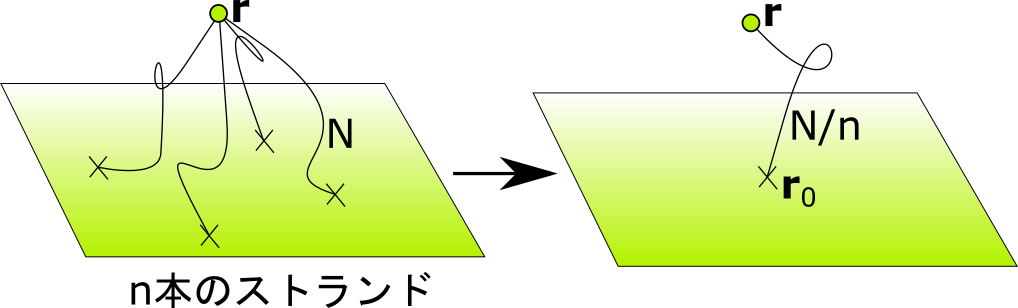
\includegraphics[width=\textwidth]{./fig/phantom-1.png}
\end{figure}
\end{block}
\column{.48\textwidth}
\begin{exampleblock}{内部の鎖が受ける変形}
\begin{itemize}
\item
システム内部の鎖の末端はガウス分布
\item
壁面に固定された末端からの変形が内部に伝達して、
\end{itemize}
\vspace{-5mm}
\tiny
\begin{align*}
&G=\xi \nu k_BT \\
&\begin{cases}
\xi_{\infty} = 1-\dfrac{2}{f} \;\; \text{System}\sim \infty \\[8pt]
\xi_{s} = \dfrac{f-1}{f+1} \;\; \text{Small Limit}
\end{cases}
\end{align*}
\vspace{-7mm}
\begin{figure}
\centering
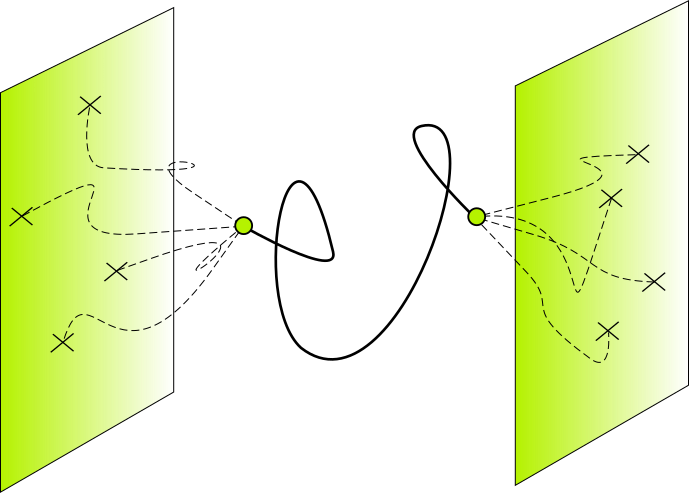
\includegraphics[width=0.6\textwidth]{./fig/phantom.png}
\end{figure}
\end{exampleblock}
\end{columns}
\end{frame}
%%%%%%%%%%%%%%%%%%%%%%%%%%%
\begin{frame}
\frametitle{シミュレーション結果(一軸伸長)}
%\vspace{-2mm}
\begin{columns}[totalwidth=\linewidth]
\column{.6\linewidth}
\vspace{-2mm}
\small
\begin{exampleblock}{$z$ 軸の伸長でのストランドの末端間距離}
\vspace{2mm}
\scriptsize
\begin{table}
\begin{tabular}{cccc} \hline
$\lambda$	& axe	& Average	&Var. 		\\ \hline \hline
			&x		&2.39		&	3.17	\\ %\cline{2-4}
$\lambda=1$	&y		&2.43		&	3.26	\\ %\cline{2-4}
			&z		&2.37		&	3.15	\\ \hline
			&x		&2.13		&	2.56	\\ %\cline{2-4}
$\lambda=2$	&y		&2.16		&	2.62	\\ %\cline{2-4}
			&z		&3.51		&	6.40	\\ \hline
			&x		&2.03		&	2.34	\\ %cline{2-4}
$\lambda=3$	&y		&2.04		&	2.37	\\
			&z		&4.88		&	11.4	\\ \hline
			&x		&1.96		&	2.19	\\
$\lambda=4$	&y		&1.97		&	2.20	\\
			&z		&6.39		&	17.6	\\ \hline
			&x 		&1.90		&	2.04	\\
$\lambda=5$	&y		&1.90		&	2.06	\\
			&z		&7.99		&	25.4	\\ \hline
\end{tabular}
\end{table}
\end{exampleblock}
\column{.35\linewidth}
\vspace{-6mm}
\begin{figure}
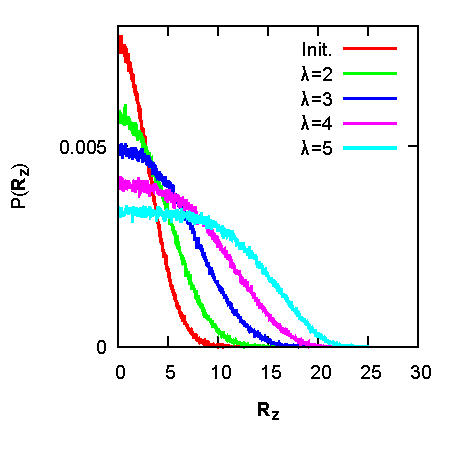
\includegraphics[width=\columnwidth]{./fig/E2E_z.pdf}
\end{figure}
\vspace{-12mm}
\begin{figure}
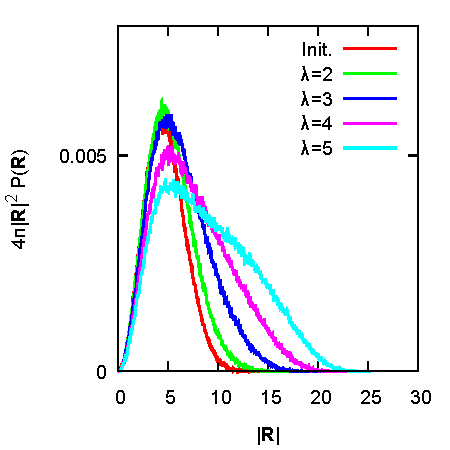
\includegraphics[width=\columnwidth]{./fig/E2E_3d.pdf}
\end{figure}
\end{columns}
\end{frame}
%%%%%%%%%%%%%%%%%%%%%%%%%%%
\begin{frame}
\frametitle{シミュレーション結果(一軸伸長)}
\small
\begin{exampleblock}{一軸伸長($10^{-4}\lambda/\tau$)}
検討対象:システム一辺当たりのユニットセル数が異なる(Cell-1d=3$\sim$6)
\vspace{-5mm}
	\begin{itemize}
	\item
	Cell-1d=3: $\xi_s$($\simeq$ 0.5 for 3-Chain) に対応した Quasi P
	\item
	セル数の増加で $\xi_{\infty}$($\simeq$ 0.33 for 3-Chain)の Phantom へ漸近
	\end{itemize}
\end{exampleblock}
\vspace{-2mm}
\begin{columns}[totalwidth=\linewidth]
\column{.48\linewidth}
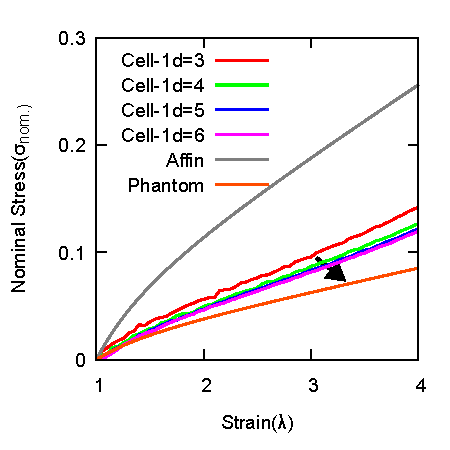
\includegraphics[width=0.9\columnwidth]{./fig/SS_affin_phantom.pdf}
\column{.48\linewidth}
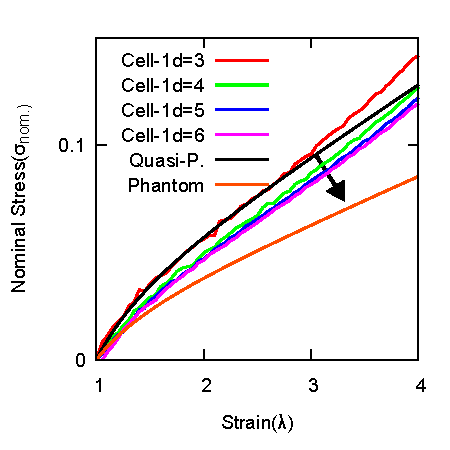
\includegraphics[width=0.9\columnwidth]{./fig/SS_all.pdf}
\end{columns}
\end{frame}
%%%%%%%%%%%%%%%%%%%%%%%%%%%
\begin{frame}
\frametitle{シミュレーション結果(一軸伸長)}
\begin{columns}[totalwidth=\linewidth]
\column{.48\linewidth}
フルチェインモデルでの伸びきり効果は以下の表式
\tiny
\begin{align*}
&\sigma_{Full} = E \dfrac{\sqrt{N}}{4\pi} \int_0^{\pi} \int_0^{2\pi} \mathcal{L}^{-1} \left( \dfrac{\lambda}{\sqrt{N}} \right) \\
&\times \dfrac{\lambda_i^2 m_i^2}{\lambda} \sin \theta \mathrm{d} \theta \mathrm{d} \phi \\
&\text{where}\;\;m_0 = \sin \theta \cos \theta,\; m_1 = \sin \theta \sin \phi, \; \\
&m_2 = \cos \theta,\;\lambda^2 = \sum_{i=0}^2 \lambda_i^2m_i^2 \notag
\end{align*}
\normalsize

Cell-1d=5 で$\xi\simeq0.4$となることを考慮して、セグメント数 $N$: $20\rightarrow60$ として換算すると、 大変形での伸びきり効果が良い一致を示した。
\vspace{-2mm}

\column{.48\linewidth}
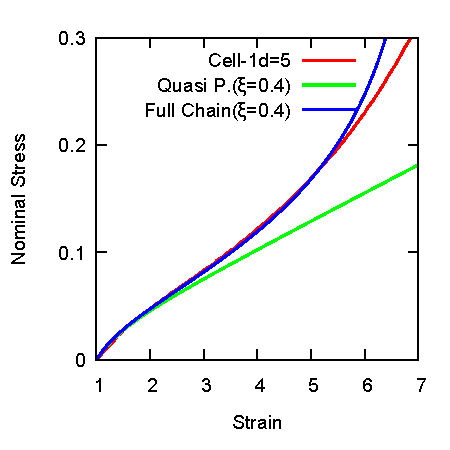
\includegraphics[width=\columnwidth]{./fig/Stretch.pdf}
\end{columns}
\end{frame}
%%%%%%%%%%%%%%%%%%
\begin{frame}
\frametitle{実験とKGネットワークとの比較}
\begin{columns}[totalwidth=1\textwidth]
\column{.5\textwidth}
\begin{itemize}
\item
$\nu \simeq 0.9\times 10^{26}$
% と概算\\
%$\rho\simeq$1, Mn$\simeq$6600
\item
$E_{af}=3\nu k_B T \simeq 1.1 [{\rm MPa}]$
\item
$E_{MR}= 2(C_1 + C_2) \simeq 0.94 [{\rm MPa}]$
\end{itemize}

\centering
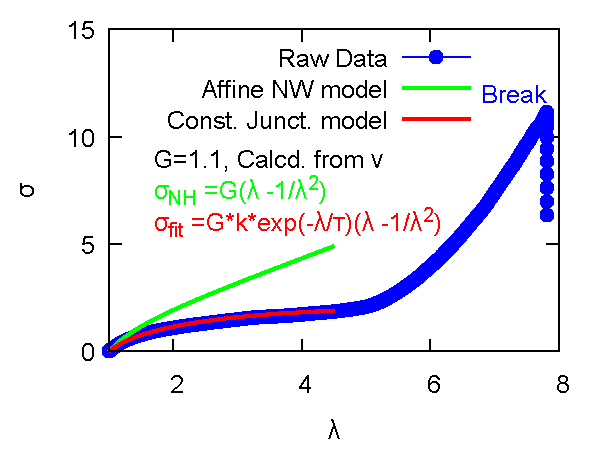
\includegraphics[width=\columnwidth]{./fig/SS_MR_6_fit.pdf}

\column{.5\textwidth}
KGネットワーク
	\begin{itemize}
	\item
	伸長に伴う変化
		\begin{itemize}
		\item
		伸長に伴いファントム的挙動へとソフトニング
		\end{itemize}
	\end{itemize}
\centering
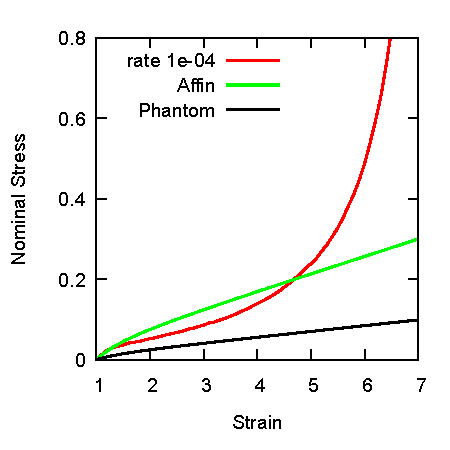
\includegraphics[width=0.8\columnwidth]{./fig/SS-2.pdf}
\end{columns}
\end{frame}
%%%%%%%%%%%%%%%%%%%
\section{おわりに}
%%%%%%%%%%%%%%%%%%%
\begin{frame}
\frametitle{おわりに}
%\vspace{-2mm}
%\begin{exampleblock}{本研究の目標とアプローチ}
%\begin{itemize}
%\item
%目標\\
%破壊耐性に優れた軽量材料の創成とその設計指針の明確化
%\item
%アプローチ
%	\begin{itemize}
%	\item
%	可逆性に優れた材料としてゴム材料を選択。
%	\item
%	構造明確なネットワークの構築のために超分子ネットワーク。
%	\item
%	既知のモデルとの\color{red}多数の整合点と、興味深い不整合\color{black}を確認。
%	\item
%	\color{red}シミュレーションでマルチスケールモデル\color{black}を構築したい。
%	\end{itemize}
%\end{itemize}
%\end{exampleblock}
\begin{block}{ランダムネットワーク構造のMDシミュレーション}
\begin{itemize}
\item
ランダムネットワーク構造の生成
	\begin{itemize}
	\item
	ストランド長をそろえた規則構造を初期構造とした。\\
	8-Chain Model を初期構造
	\item
	各ノードごとにランダムな結合性を導入\\
	トポロジーモデルを用いて、ラプラシアン行列で結合性を評価しながらランダム性を導入
	\item
	ホモポリマーメルトと同様な分布関数のランダムネットワーク構造を生成できた。
	\end{itemize}
\item
ランダムネットワーク構造のMDシミュレーション
	\begin{itemize}
	\item
	システムサイズ依存でのファントムネットワークの挙動を確認
	\item 
	伸びきり効果もシステムサイズ依存で再現
	\end{itemize}
\end{itemize}
\end{block}
\end{frame}
%%%%%%%%%%%%%%%%%%%%%%%%%%%%%%%%%%%%%%%%%%%%%%%%
\appendix
%%%%%%%%%%%%%%%%%
\begin{frame}
\LARGE{補足資料}
\end{frame}
%%%%%%%%%%%%%%%%
%%%%%%%%%%%%%%%%%%%%%%%%%%
\section{マルチスケールと物性}
%%%%%%%%%%%%%%%%%%%%%%%%%%%%
\begin{frame}
\frametitle{マルチスケールと物性}
\href{http://j-parc.jp/ja/topics/2015/Pulse151112.html}{J-PARCの広報サイト}から引用。
\small
『SPring-8・J-PARC・スーパーコンピュータ「京」を連携活用させたタイヤ用新材料開発技術「ADVANCED 4D NANO DESIGN」を確立』
\centering
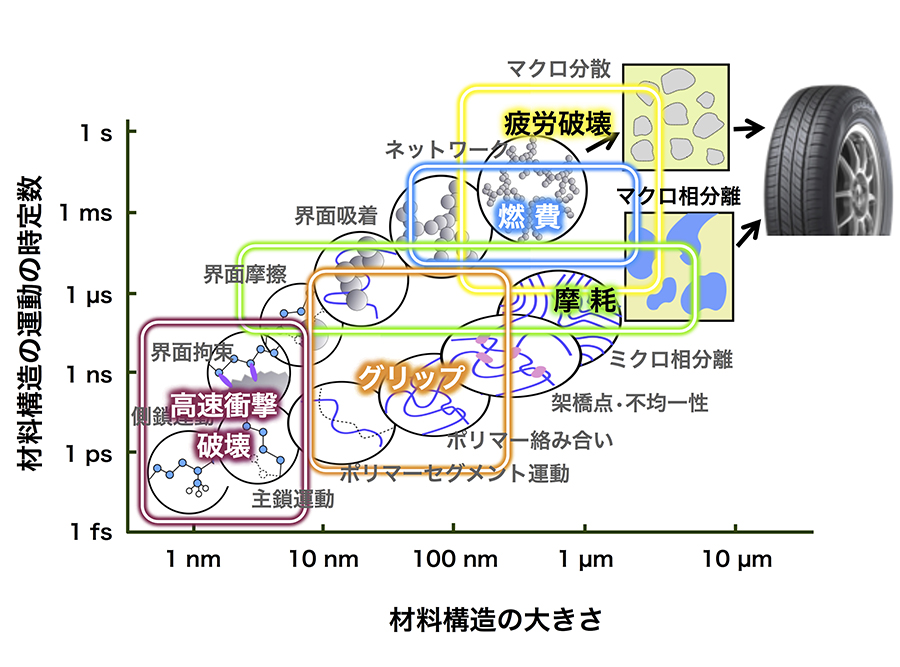
\includegraphics[width=75mm]{./fig/press151112_02.jpg}
\end{frame}
%%%%%%%%%%%%%%%%%%%%%%%%%%%%
\begin{frame}
\frametitle{スケールと特徴的構造}
\href{http://j-parc.jp/ja/topics/2015/Pulse151112.html}{J-PARCの広報サイト}から引用。
\small
『SPring-8・J-PARC・スーパーコンピュータ「京」を連携活用させたタイヤ用新材料開発技術「ADVANCED 4D NANO DESIGN」を確立』
\centering
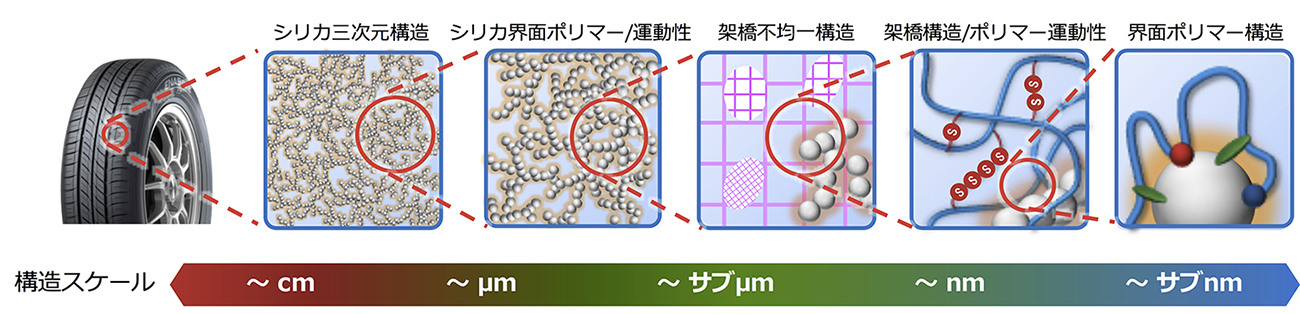
\includegraphics[width=105mm]{./fig/press151112_03.jpg}
\end{frame}


%%%%%%%%%%%%%%%%%%%%%%%%%%%%%%%%%%
\begin{frame}
\frametitle{これまでにできていたこと}
\begin{columns}[totalwidth=1\textwidth]
\column{.48\textwidth}
\begin{block}{合成ベースのアプローチ}
\begin{itemize}
\item
一軸伸長
	\begin{itemize}
	\item
	伸長初期はアフィン応答
	\item
	ファントム挙動へとシアソフトニング
	\end{itemize}
\item
ヒステリシス特性
	\begin{itemize}
	\item
	大きなヒステリシス挙動
	\item
	ファントムモデルへの漸近
	\item
	迅速な変形回復
	\end{itemize}
\end{itemize}
\end{block}

\column{.48\textwidth}
\begin{block}{シミュレーションのアプローチ}
\begin{itemize}
\item
ネットワーク構造
	\begin{itemize}
	\item
	ダイヤモンド構造の狙い通りの規則構造
	\item
	末端間距離が揺らぐ構造
	\end{itemize}
\item
一軸伸長
	\begin{itemize}
	\item
	アフィンネットワークとしての振る舞い
	\item
	伸びきり挙動もほぼ理論通り
	\end{itemize}
\end{itemize}
\end{block}
\end{columns}

\begin{alertblock}{やりたいこと}
\begin{itemize}
\item
ファントム的な挙動をシミュレーションで再現したい。
\item
結晶性のないポリマーで粘弾性特性を明確にしたい
\end{itemize}
\end{alertblock}
\end{frame}
%%%%%%%%%%%%%%%%%%%%%%%%%%%%%%%%%%%%%%
\section{ファントムネットワークの理論}
%%%%%%%%%%%%%%%%%%%%%%%%%%%%%%%%%%%%%%
%%%%%%%%%%%%%%%%%%%%%%%%%%%%%%%%%%%%%%%%%%%%%%
\subsection{ファントムネットワークの振る舞い}
%%%%%%%%%%%%%%%%%%%%%%%%%%%%%%%%%%%%%%%%%%%%%%
%%%%%%%%%%%%%%
\begin{frame}
\frametitle{ファントムネットワークのゆらぎ}

\begin{columns}[totalwidth=1\textwidth]
\column{.47\textwidth}
\scriptsize
\begin{block}{ゆらぎの入ったポテンシャル}
ストランドの末端間ベクトル $\bm{R}_{nm}$ を、\\架橋点の位置ベクトル $\bm{r}_n$ を用いて、
\vspace{-3mm}
\begin{equation*}
\bm{R}_{nm} \equiv \bm{r}_n-\bm{r}_m
\end{equation*}

系のポテンシャルエネルギーは、
\vspace{-3mm}
\begin{equation*}
U=\dfrac{k}{2} \sum_{\langle nm \rangle} \bm{R}_{nm}^2
\end{equation*}

これは、自然長で決まる定数項と、ゆらぎに起因した第二項に分割でき、その和で以下となる。
\vspace{-3mm}
\begin{equation*}
U=\dfrac{k}{2} \sum_{\langle nm \rangle} {\bm{R}_{nm}^{(0)}}^2 + \dfrac{k}{2} \sum_{\langle nm \rangle} \Delta \bm{R}_{nm}^2
\end{equation*}
\end{block}

\column{.47\textwidth}
\scriptsize
\begin{block}{アンサンブル平均の二つの表式}
\vspace{-5mm}
\begin{align*}
 \begin{cases}
	\langle U \rangle = N_{strands} \dfrac{k}{2} \langle \Delta \bm{R}^2 \rangle \\
	\langle U \rangle = 3(N_{nodes}-1) \dfrac{1}{2} k_B T
 \end{cases}
\end{align*}
なお、第二式は等分配側より導出した。
\end{block}

\begin{exampleblock}{ファントムネットワークでのゆらぎ}
架橋点数 $N_{nodes}$、架橋点官能基数 $f$ とすれば、規則格子での一般式として、
\vspace{-3mm}
\begin{equation*}
\langle \Delta \bm{R}^2 \rangle = \dfrac{3k_B T}{k} \dfrac{2}{f} \left( 1-\dfrac{1}{N_{nodes}} \right)
\end{equation*}

適切な条件で、ストランドの自然長 $R_0$\\
を用いて、
\vspace{-3mm}
\begin{equation*}
\color{red}
\langle \Delta \bm{R}^2 \rangle = \dfrac{2}{f} R_0^2
\end{equation*}
\vspace{-6mm}
\end{exampleblock}

\end{columns}

\end{frame}


%%%%%%%%%%%%%%%%%
\begin{frame}
\frametitle{ファントムネットワークの振る舞い}

\begin{columns}[totalwidth=1\textwidth]
\column{.47\textwidth}
\scriptsize
\begin{block}{ストランドの末端間距離}
ストランドの末端間距離の分布関数は、畳み込み積分の形で、
\vspace{-3mm}
\begin{equation*}
\Omega(\bm{R}) = \Phi(\bar{\bm{R}}) + \Psi(\bm{\Delta R})
\end{equation*}

ダイヤモンド構造でのストランド末端間距離の $x$ 成分の分布関数 $P_{strand}(x)$ は、\vspace{-3mm}
\begin{align*}
P_{strand}(x) 
&= \dfrac{1}{2}\dfrac{1}{\sqrt{2\pi}\Delta_{\lambda}^x} \\
&\times \left[ \exp\left(-\dfrac{(x-X_{\lambda})^2}{2(\Delta_{\lambda}^x)^2} \right) \right. \\
&\quad \left. + \exp\left(-\dfrac{(x+X_{\lambda})^2}{2(\Delta_{\lambda}^x)^2} \right) \right]
\end{align*}
なお、$X_{\lambda}$、$\Delta_{\lambda}^x$ は、伸長比 $\lambda$ である時の、ストランド長及びゆらぎの $x$ 成分を表す。
\end{block}

\column{.47\textwidth}
\scriptsize
\begin{block}{ずり弾性率 $G_{ph}$}
ファントムネットワークでのずり弾性率 $G_{ph}$ は、以下の表式で表される。
\vspace{-3mm}
\begin{align*}
G_{ph} &= \dfrac{1}{3} \dfrac{1}{V} \left. \dfrac{d^2 F_{ph}}{d \lambda^2} \right|_{\lambda = 1}\\
&=\dfrac{\langle R_{strand}^2 \rangle}{\langle R_0^2 \rangle} \nu k_B T
\end{align*}
ここで、$\nu$ は、ストランドの数密度である。

\vspace{3mm}
ダイヤモンド構造のように規則構造からなるネットワークにおいて、各ストランド長がガウス鎖の二乗平均末端距離となるようにシステムサイズを設定した場合、$\langle R_{strand}^2 \rangle = \langle R_0^2 \rangle$ であるので、
\vspace{-3mm}
\begin{align*}
\color{red}
G_{ph}= \nu k_B T
\end{align*}

\end{block}
\end{columns}
\end{frame}
%%%%%%%%%%%%%%%%%%%%%%
\subsection{伸長時の振る舞い}
%%%%%%%%%%%%%%%%%
\begin{frame}
\frametitle{伸長時($\lambda =2$)の振る舞い}

\begin{columns}[T, totalwidth=1\linewidth]
\column{.49\linewidth}
%\vspace{-3mm}
伸長時 $\lambda =2$
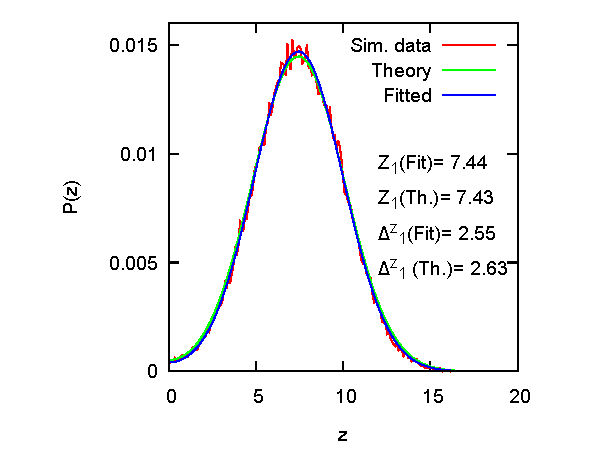
\includegraphics[width=\textwidth]{./fig/L2_Rz.pdf}
\column{.49\linewidth}
%\vspace{-3mm}
未伸長
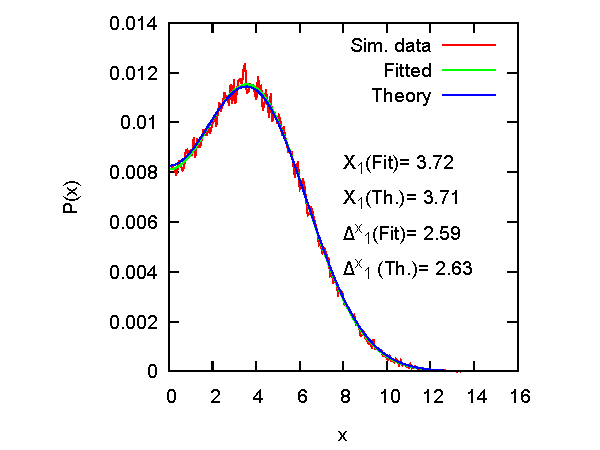
\includegraphics[width=\textwidth]{./fig/L1_Rx.pdf}
\end{columns}
\small
\begin{exampleblock}{未伸長との比較}
\begin{itemize}
\item
$z$ 軸方向への伸長の一次元での末端間距離は正確に二倍になった。
\item
ゆらぎは、理論的には不変なのであるが、5 \% 程度減少していた。
\end{itemize}
\end{exampleblock}
\end{frame}


%%%%%%%%%%%%%%%%%%%%%%%%%%%%%%%%%%%%%%%%%%%%%
\subsection{規則ネットワーク構造での検討結果}
%%%%%%%%%%%%%%%%%%%%%%%%%%%%%%%%%%%%%%%%%%
\begin{frame}
\frametitle{規則ネットワーク構造のMD シミュレーション}
OCTA 上の Cognac により、MD シミュレーションを実施。
\begin{columns}[T, totalwidth=1\linewidth]
\column{.5\linewidth}
\begin{block}{\large シミュレーション条件}
	\begin{itemize}
	\item
	KG モデル
	\item
	構造:ダイヤモンド構造
	\item
	緩和条件:\\
	NPTで所定の密度 $\Rightarrow$ NVT
	\end{itemize} 
\end{block}
\vspace{5mm}
\centering
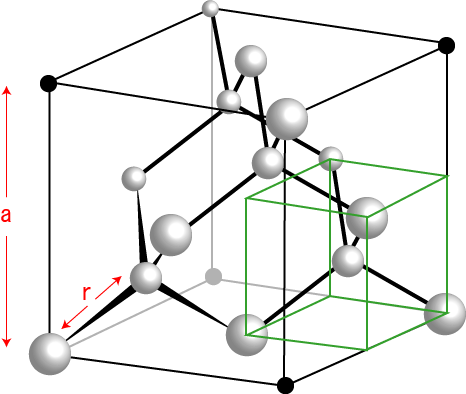
\includegraphics[width=0.6\columnwidth]{./fig/dia_green_2.png}
\column{.01\linewidth}
\column{.45\linewidth}
初期状態($\rho \simeq 0.2$)
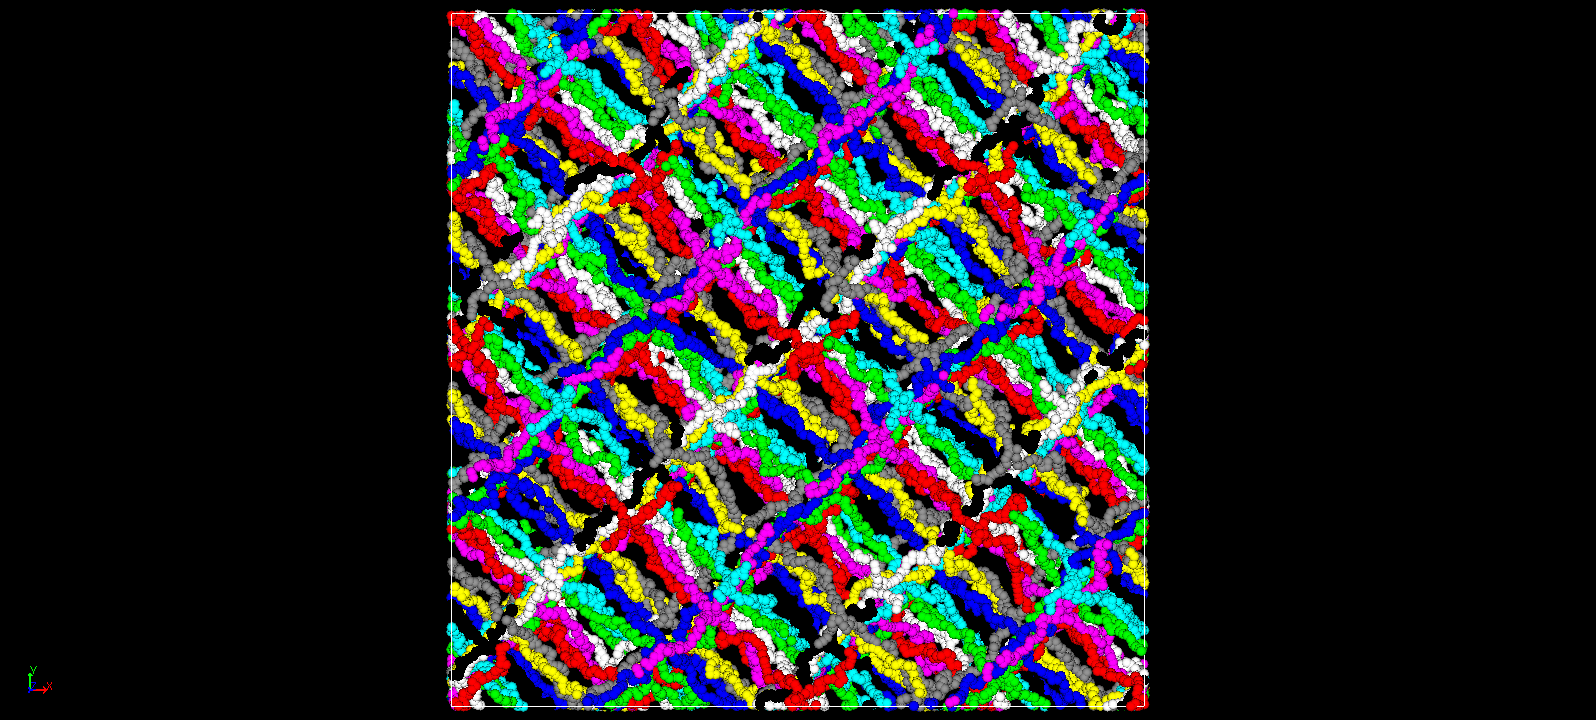
\includegraphics[width=\columnwidth]{./fig/Init.png}
\vspace{-3mm}
\begin{center}
$\Downarrow$ NPT
\end{center}
\vspace{-3mm}
初期緩和後($\rho =0.85$)
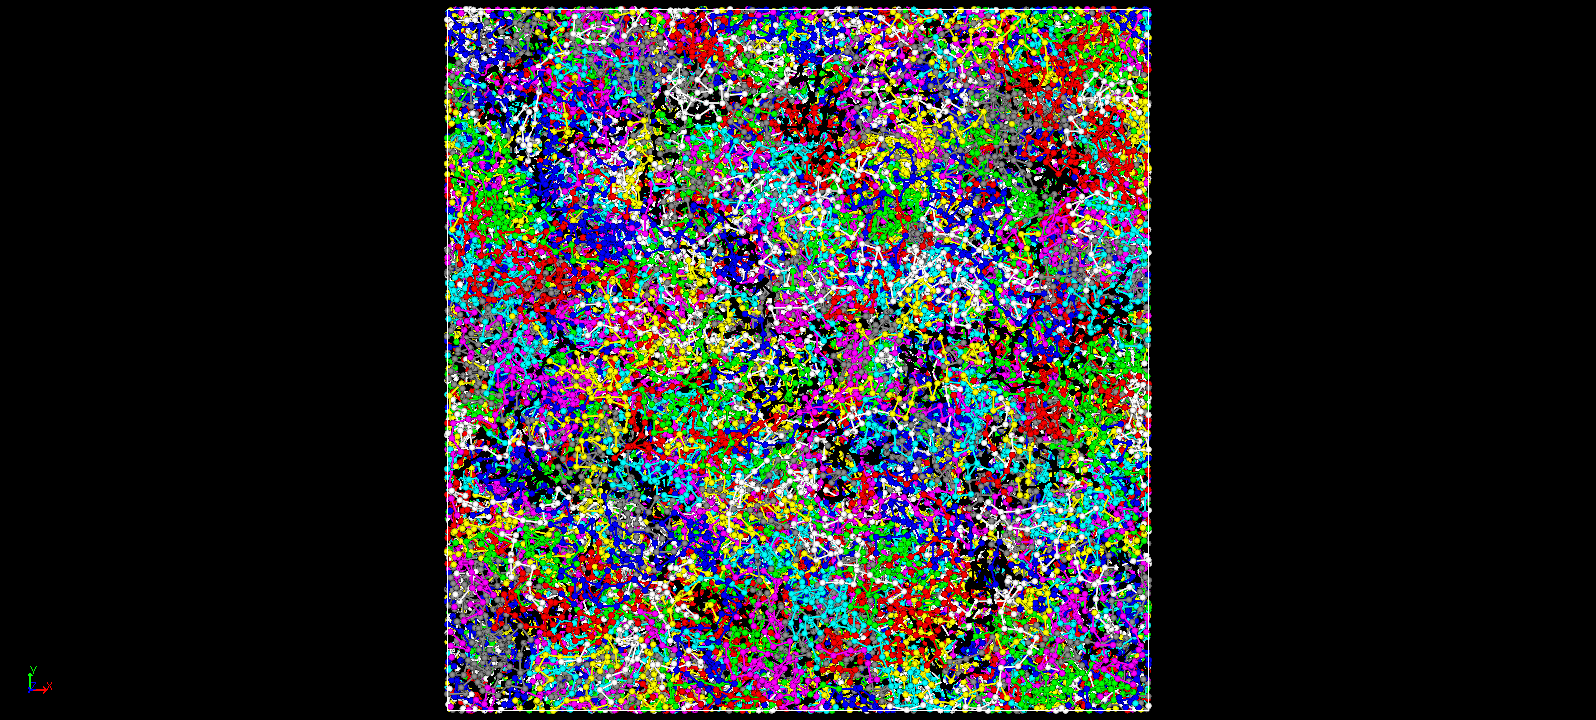
\includegraphics[width=\columnwidth]{./fig/after.png}
\end{columns}
\end{frame}
%%%%%%%%%%%%%%%%%%%%%%%%%%%%%%%%%%%%%%
\begin{frame}
\frametitle{クーン長としての換算}
\begin{columns}[totalwidth=1\textwidth]
\column{.48\textwidth}
\small
\begin{alertblock}{KG 鎖を自由連結鎖に換算}
\begin{itemize}
\item
KG 鎖のアングルは、$\simeq74$
\item
このストランドのクーンセグメント数は $N_K\simeq16.6$ と換算
\item
伸びきり効果が発現する伸長比が低下。
\item
フィッティングでは、$N\simeq21$
\end{itemize}
\end{alertblock}
\footnotesize
4-Chain model
\tiny
\begin{align*}
\sigma_{8ch}
	&= \dfrac{\nu k_B T }{3}\sqrt{N}
			\mathcal{L}^{-1} \left(\dfrac{\lambda_{chain}}{ \sqrt{N} } \right)
			\dfrac{\lambda-\dfrac{1}{\lambda^2}}{\lambda_{chain}} 
\end{align*}
\column{.5\textwidth}
\centering
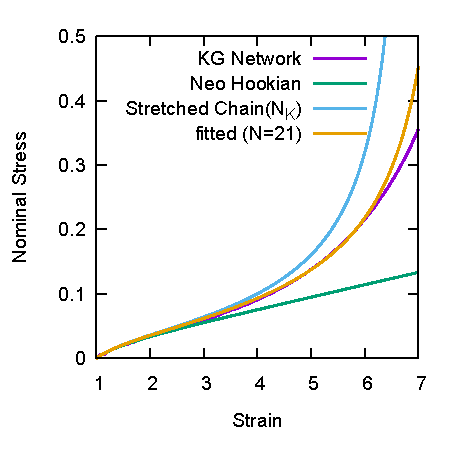
\includegraphics[width=\columnwidth]{./fig/SS_Kuhn.pdf}
\end{columns}
\end{frame}
%%%%%%%%%%%%%%%%%%%%%%%%%%
\begin{frame}
\frametitle{線形粘弾性スペクトル}
\vspace{-2mm}
\begin{columns}[totalwidth=1\textwidth]
\column{.48\textwidth}
\begin{block}{応力緩和スペクトル}
\begin{itemize}
\small
\item
Green-Kubo form. により、応力緩和スペクトルを算出
\end{itemize}
\end{block}
\centering
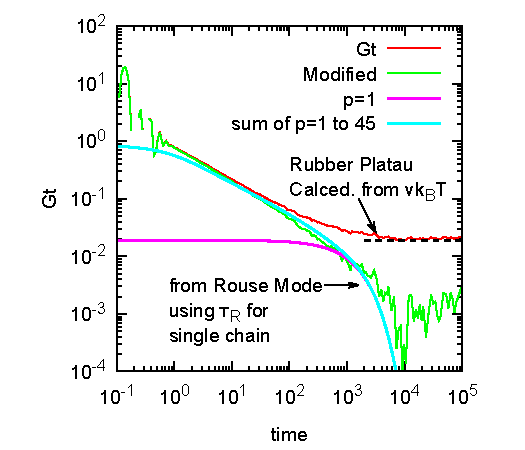
\includegraphics[width=\columnwidth]{./fig/Gt_loglog.pdf}
\column{.02\textwidth}
\column{.48\textwidth}
\begin{exampleblock}{動的粘弾性スペクトル}
\begin{itemize}
\small
\item
応力緩和スペクトルより算出
\item
ずり変形より算出(離散値)
\end{itemize}
\end{exampleblock}
\centering
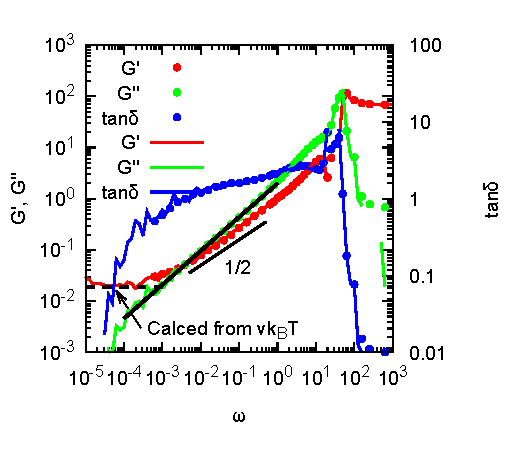
\includegraphics[width=\columnwidth]{./fig/N_44_Freq_Sweep.pdf}
\end{columns}
ストランドと同等な自由鎖(N=46)のラウス緩和(最長ラウス緩和時間 $\tau_R = 2700$)についても示している。
\end{frame}
%%%%%%%%%%%%%%%%%%%%%%%%%%
\begin{frame}
\frametitle{力学的ヒステリシス}
\begin{columns}[totalwidth=1\textwidth]
\column{.48\textwidth}
最長緩和時間の逆数程度のオーダーである変形速度($5E^{-4}\lambda/\tau$)での一軸伸長において、任意の変形量($\lambda = 1.2, 1.5, 2.0, 2.5$)まで伸長した後に同等の変形速度で圧縮を行い、力学的ヒステリシスを測定した\\
また、伸長速度を遅くすることにより、ヒステリシス強度が減少することも確認できた。
\column{.48\textwidth}
\centering
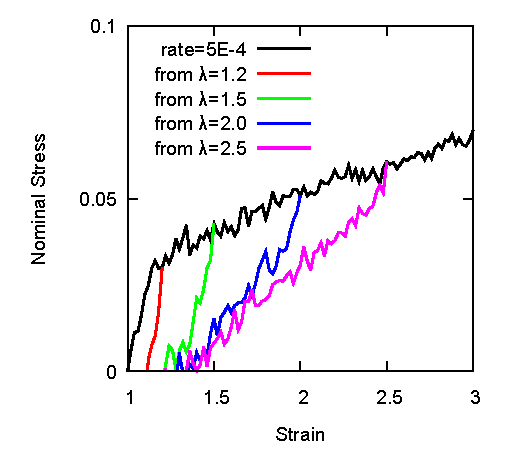
\includegraphics[width=\textwidth]{./fig/N44_rev_SS.pdf}
\end{columns}
\end{frame}
%%%%%%%%%%%%%%%%%%%%%%%%%%%%
\section{その他}
%%%%%%%%%%%%%%%
\begin{frame}
%[shrink squeeze]
\frametitle{高分子材料の疲労と破壊}
\begin{columns}[totalwidth=1\textwidth]
\column{.6\textwidth}
ガラス状態の高分子材料では、
\begin{block}{破壊のモード(巨視的)}
脆性破壊 $\Leftrightarrow$ 延性破壊\\
脆性破壊は、降伏前にミクロなクラックが進展した破壊とも考えられる。
\end{block}
\column{.4\textwidth}
	\centering
	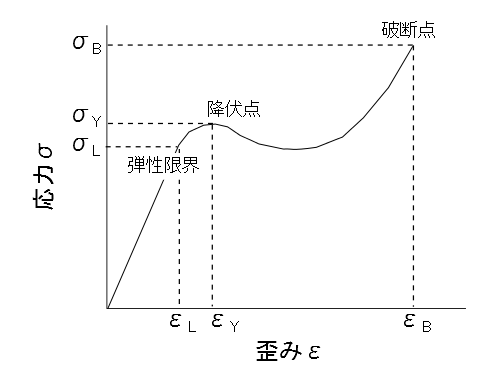
\includegraphics[width=\textwidth]{./fig/S_S_Curve.png}
\end{columns}
\begin{exampleblock}{降伏と劣化}
	\begin{itemize}
	\item
	靭性向上のため
	\begin{itemize}
		\item
		{\color{red} 局所的な降伏}が必須。(クレイズのような局所的な破壊も含む)
		\item 
		一般に、高分子材料の{\color{red} 降伏は不可逆}。
	\end{itemize}
	\item
	降伏による劣化
		\begin{itemize}
			\item 
			降伏 $\Leftrightarrow$ {\color{red} 本質的には、少しずつ破壊。}
			\item
			{\color{red} 破壊領域への水分の浸透 $\Leftarrow$ 長期耐久性の欠如}
		\end{itemize}
	\end{itemize}
\end{exampleblock}
\end{frame}
%%%%%%%%%%%%%%%%%%%%%%%%%%%%
\begin{frame}
\frametitle{ヒステリシス特性(実験系の例)}
\begin{columns}[totalwidth=1\textwidth]
\column{.4\textwidth}
{\Large 実験系の例}
\small
\begin{block}{実験条件}
\begin{itemize}
\item
チャック間距離:20mm
\item
伸長速度:10mm/min.
\end{itemize}
\end{block}
\begin{alertblock}{除荷時の挙動}
\begin{itemize}
\item
早い構造緩和
\item
ファントムモデルへの漸近
\end{itemize}
\end{alertblock}
\column{.01\textwidth}
\column{.58\textwidth}
\centering
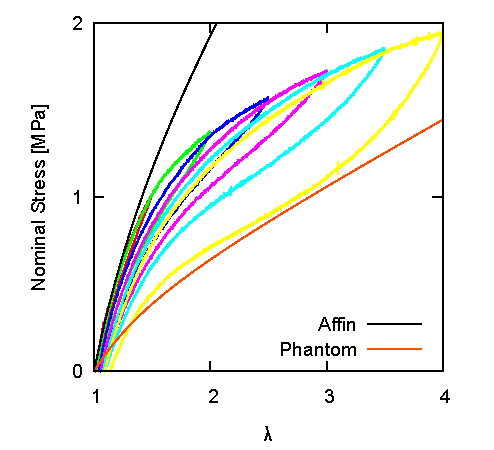
\includegraphics[width=\textwidth]{./fig/Hysteresis_10mm.pdf}
\end{columns}
\end{frame}
%%%%%%%%%%%%%%%%%%%%%%%%%%%%%%%%%%%%%%%%%%%%%%%%
\begin{frame}
\frametitle{架橋点近傍の拘束状態に基づく二つのモデル}
\begin{columns}[totalwidth=1\textwidth]
\column{.5\textwidth}
ストランドと架橋点の模式図
%\centering
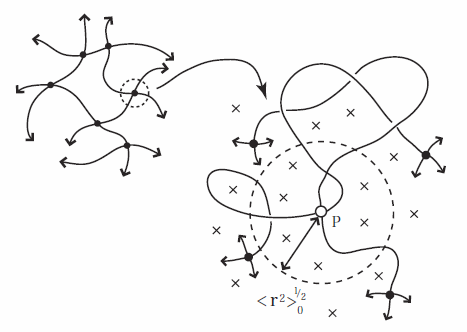
\includegraphics[width=\textwidth]{./fig/JP_vicinity.png}
架橋点はストランド経由で直接連結した架橋点(図中の黒丸)以外の、近接する多数のストランド及び架橋点(図中の×)に囲まれている。
\column{.5\textwidth}
\begin{itemize}
\item
``Affine NW Model''\\
架橋点は周辺に強く拘束され巨視的変形と相似に移動。\\(Affine 変形)
\footnotesize
\begin{equation*}
G=\nu k_B T
\end{equation*}
\normalsize
$\nu$ は、ストランドの数密度
\item
``Phantom NW Model''\\
架橋点が大きく揺らぎ、実効的なずり弾性率($G$)が低下。
\footnotesize
\begin{align*}
G&=\xi \nu k_B T \\
\xi&= 1 -\dfrac{2}{f}
\end{align*}
\normalsize
$f$ は架橋点の分岐数
\end{itemize}
\end{columns}
\end{frame}
%%%%%%%%%%%%%%%%%%%
\begin{frame}
\frametitle{架橋点の近傍}
\centering
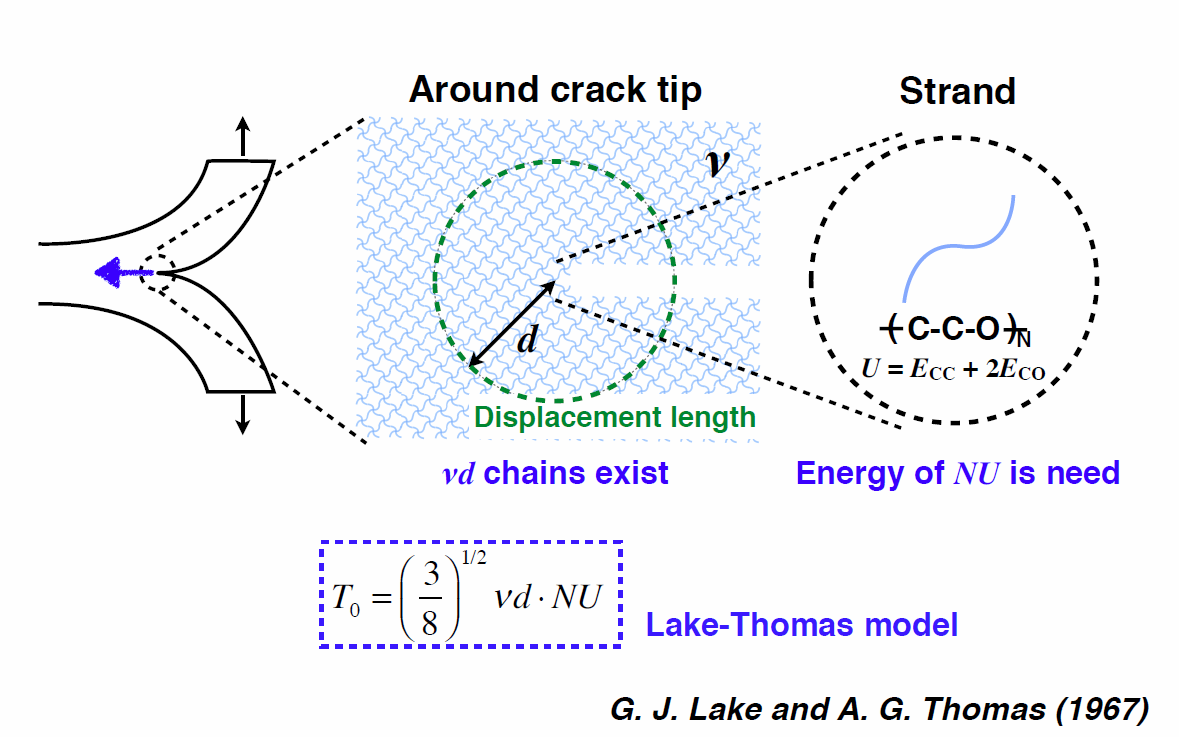
\includegraphics[width=100mm]{./fig/Lake_Thomas.png}
\end{frame}
%%%%%%%%%%%%%%%%%
\begin{frame}
\frametitle{ゴムの破壊と粘弾性}
\begin{block}{ゴムの破壊}
ゴムの破壊は大変形を伴うにもかかわらず、時間温度換算則が成立する例が多数報告されている。
\end{block}
\begin{columns}[totalwidth=1\textwidth]
\column{.48\textwidth}
ゴムの亀裂先端近傍での大変形
\centering
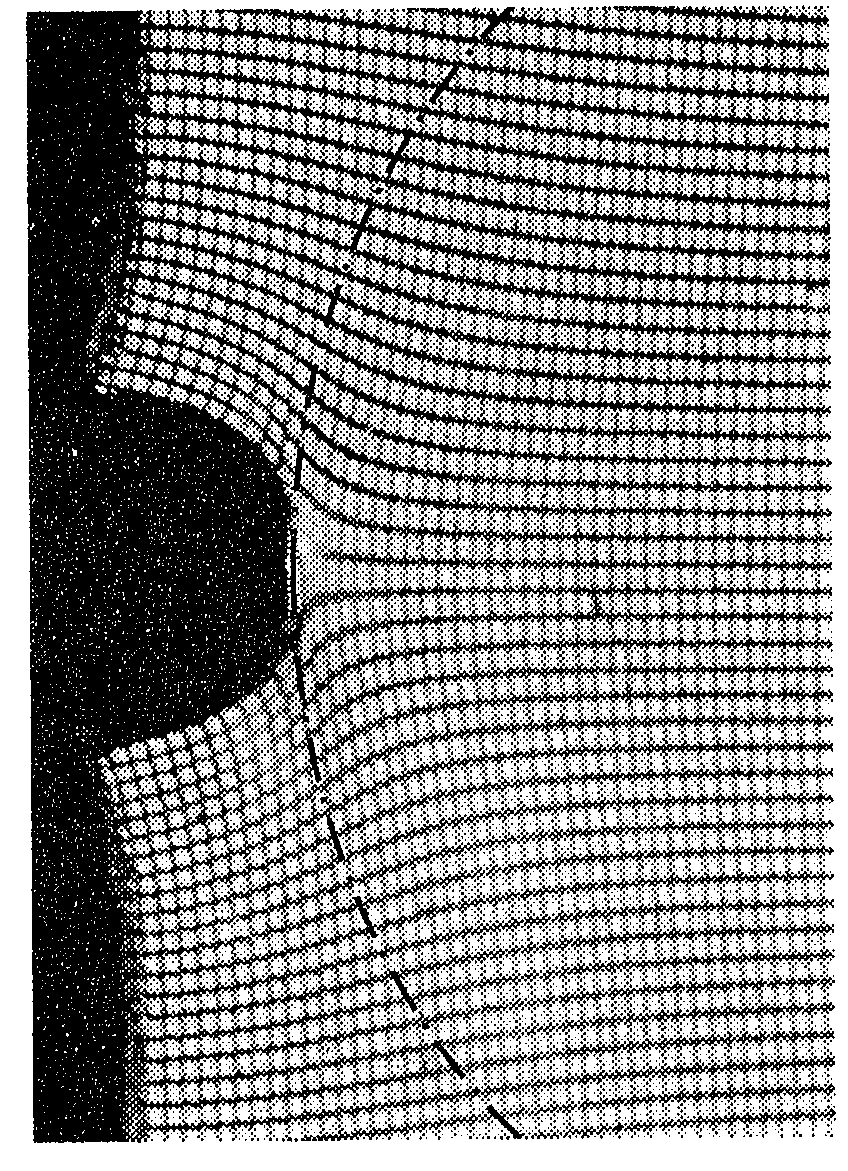
\includegraphics[width=.6\textwidth]{./fig/rubber_crack.png}
\column{.48\textwidth}
時間温度換算則の成立
\centering
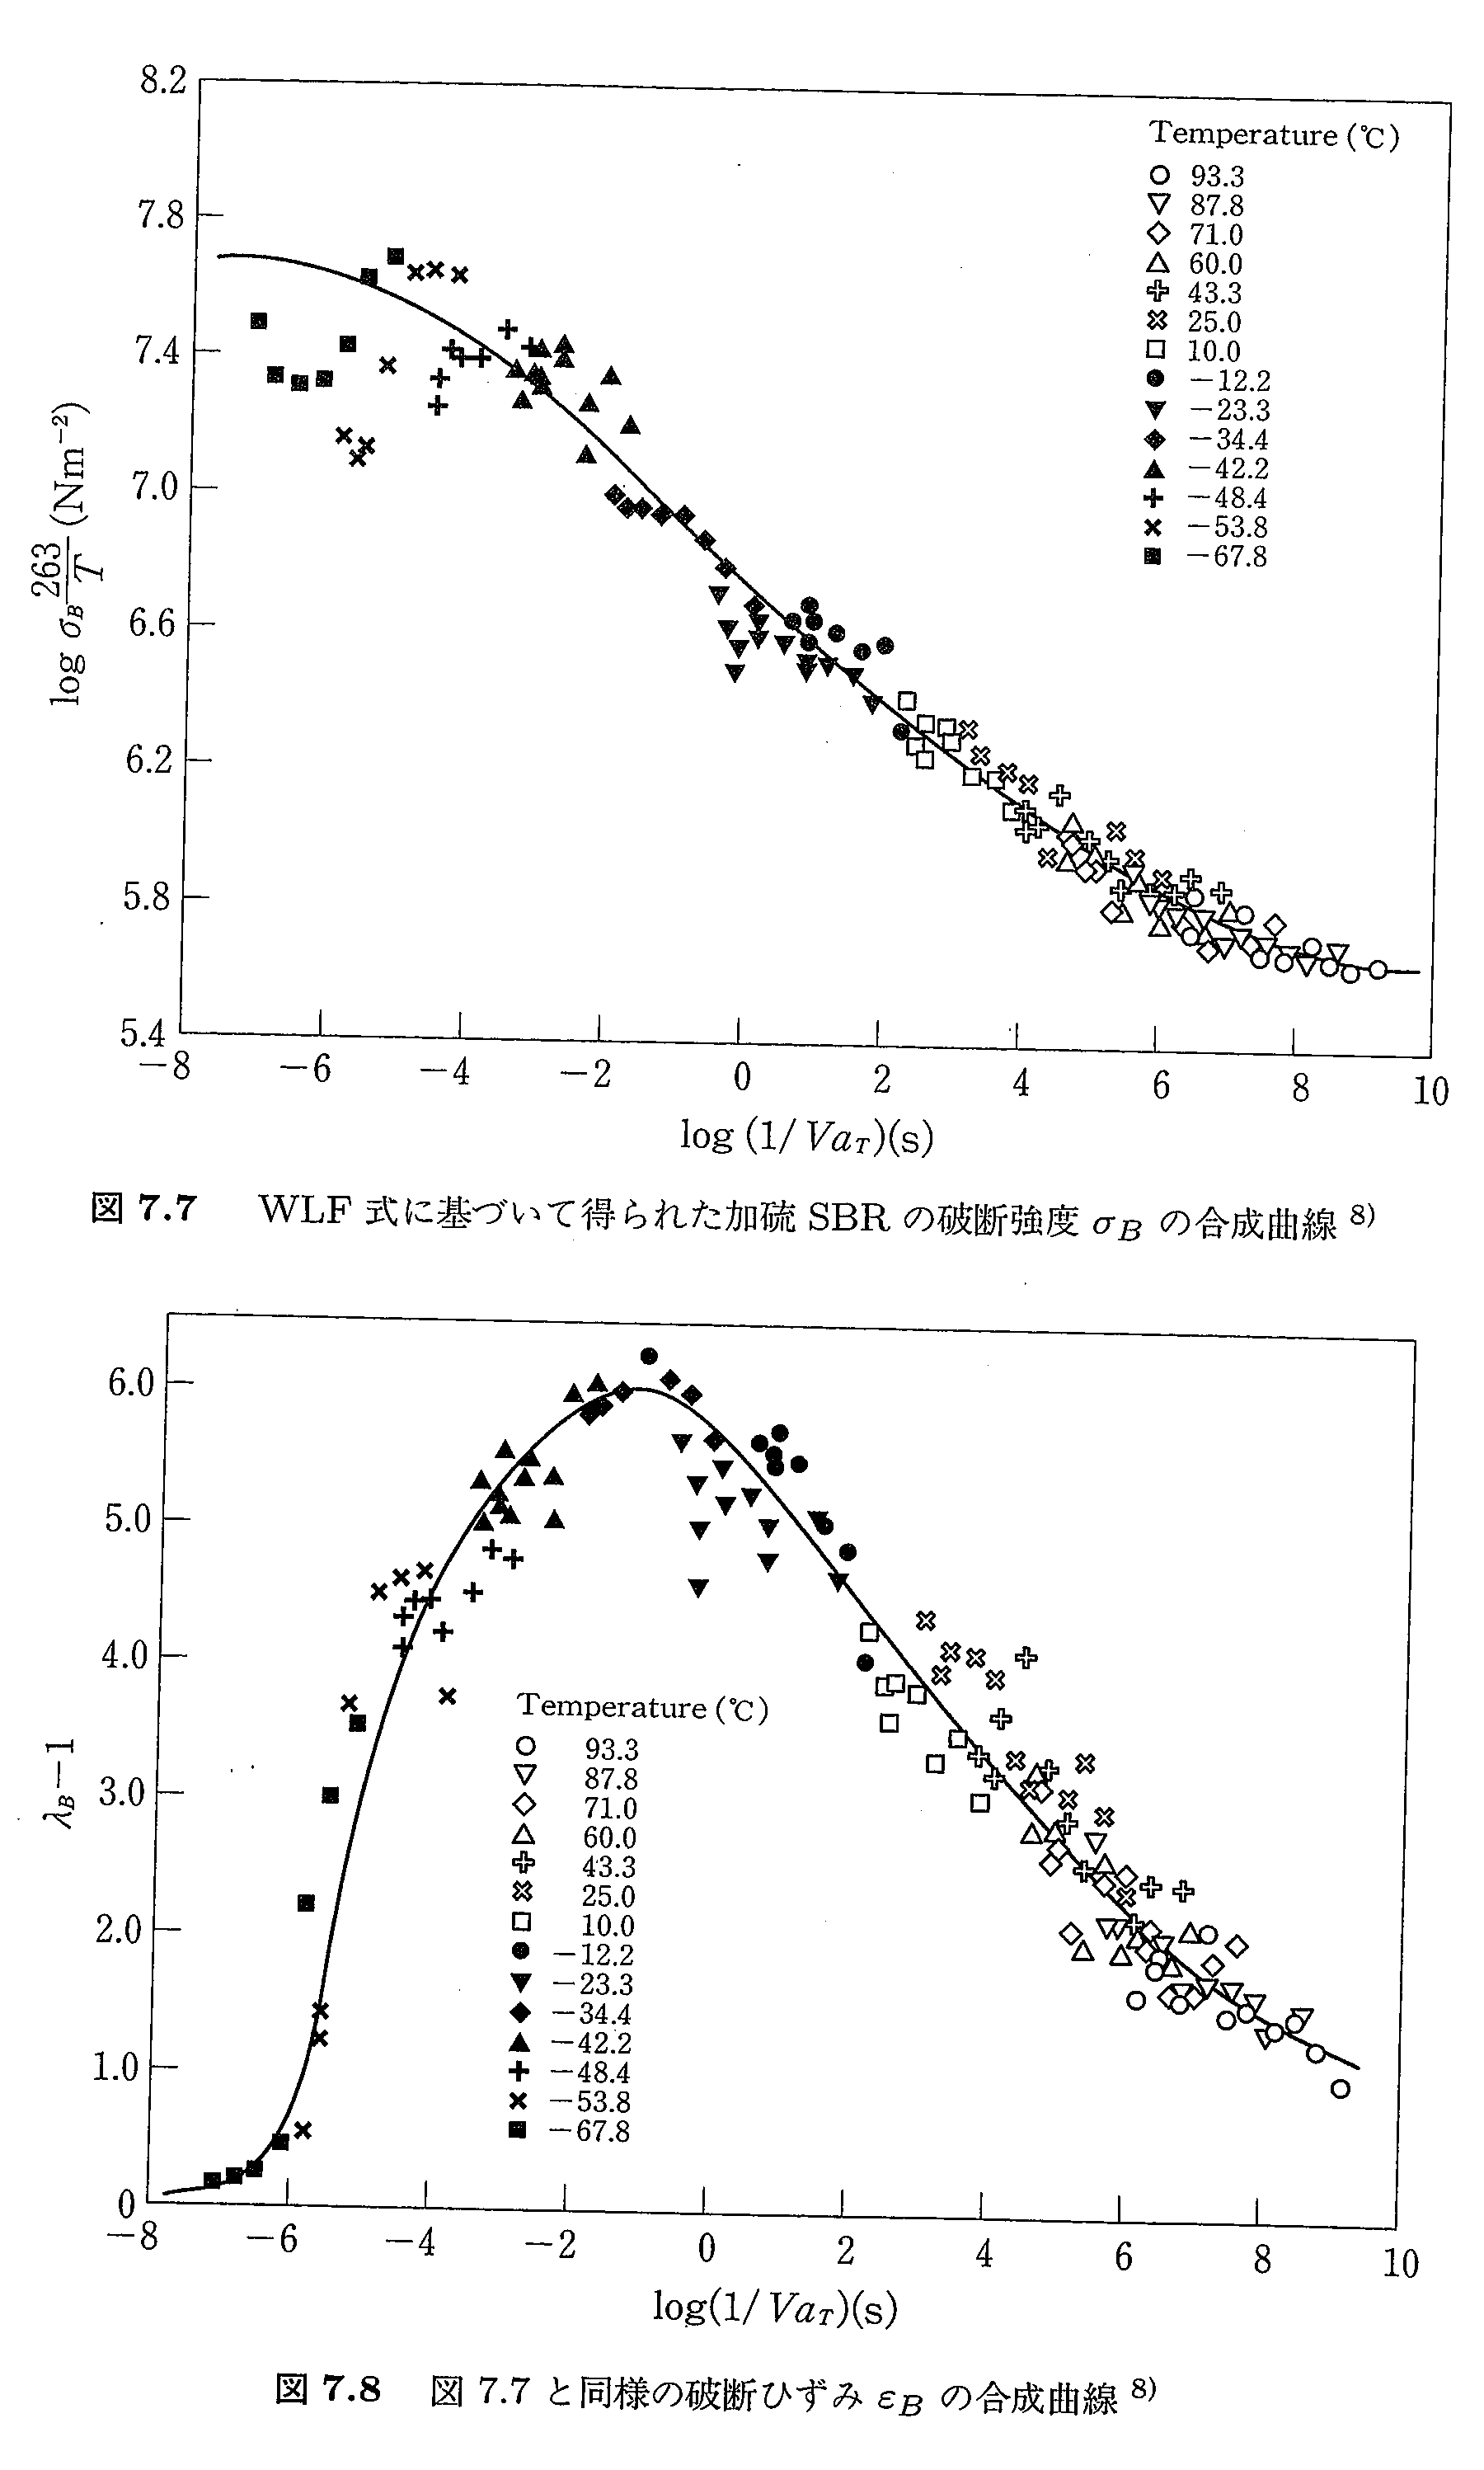
\includegraphics[width=.5\textwidth]{./fig/Time_Temp.png}
\end{columns}
\end{frame}
%%%%%%%%%%%%%%%%%
\begin{frame}
\frametitle{引き裂きエネルギーの時間温度依存}
\begin{columns}[totalwidth=1\textwidth]
\column{.48\textwidth}
粘弾性効果の極限\\
高温・低速
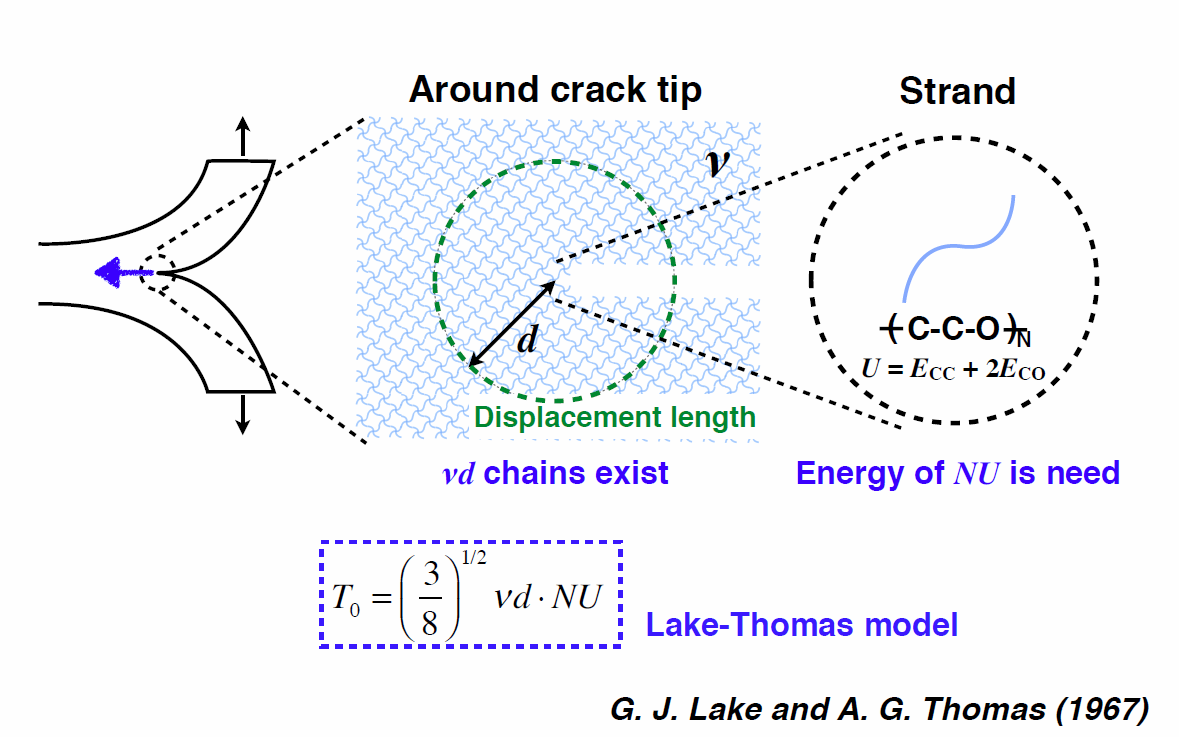
\includegraphics[width=\textwidth]{./fig/Lake_Thomas.png}
\column{.48\textwidth}
判りやすい依存性
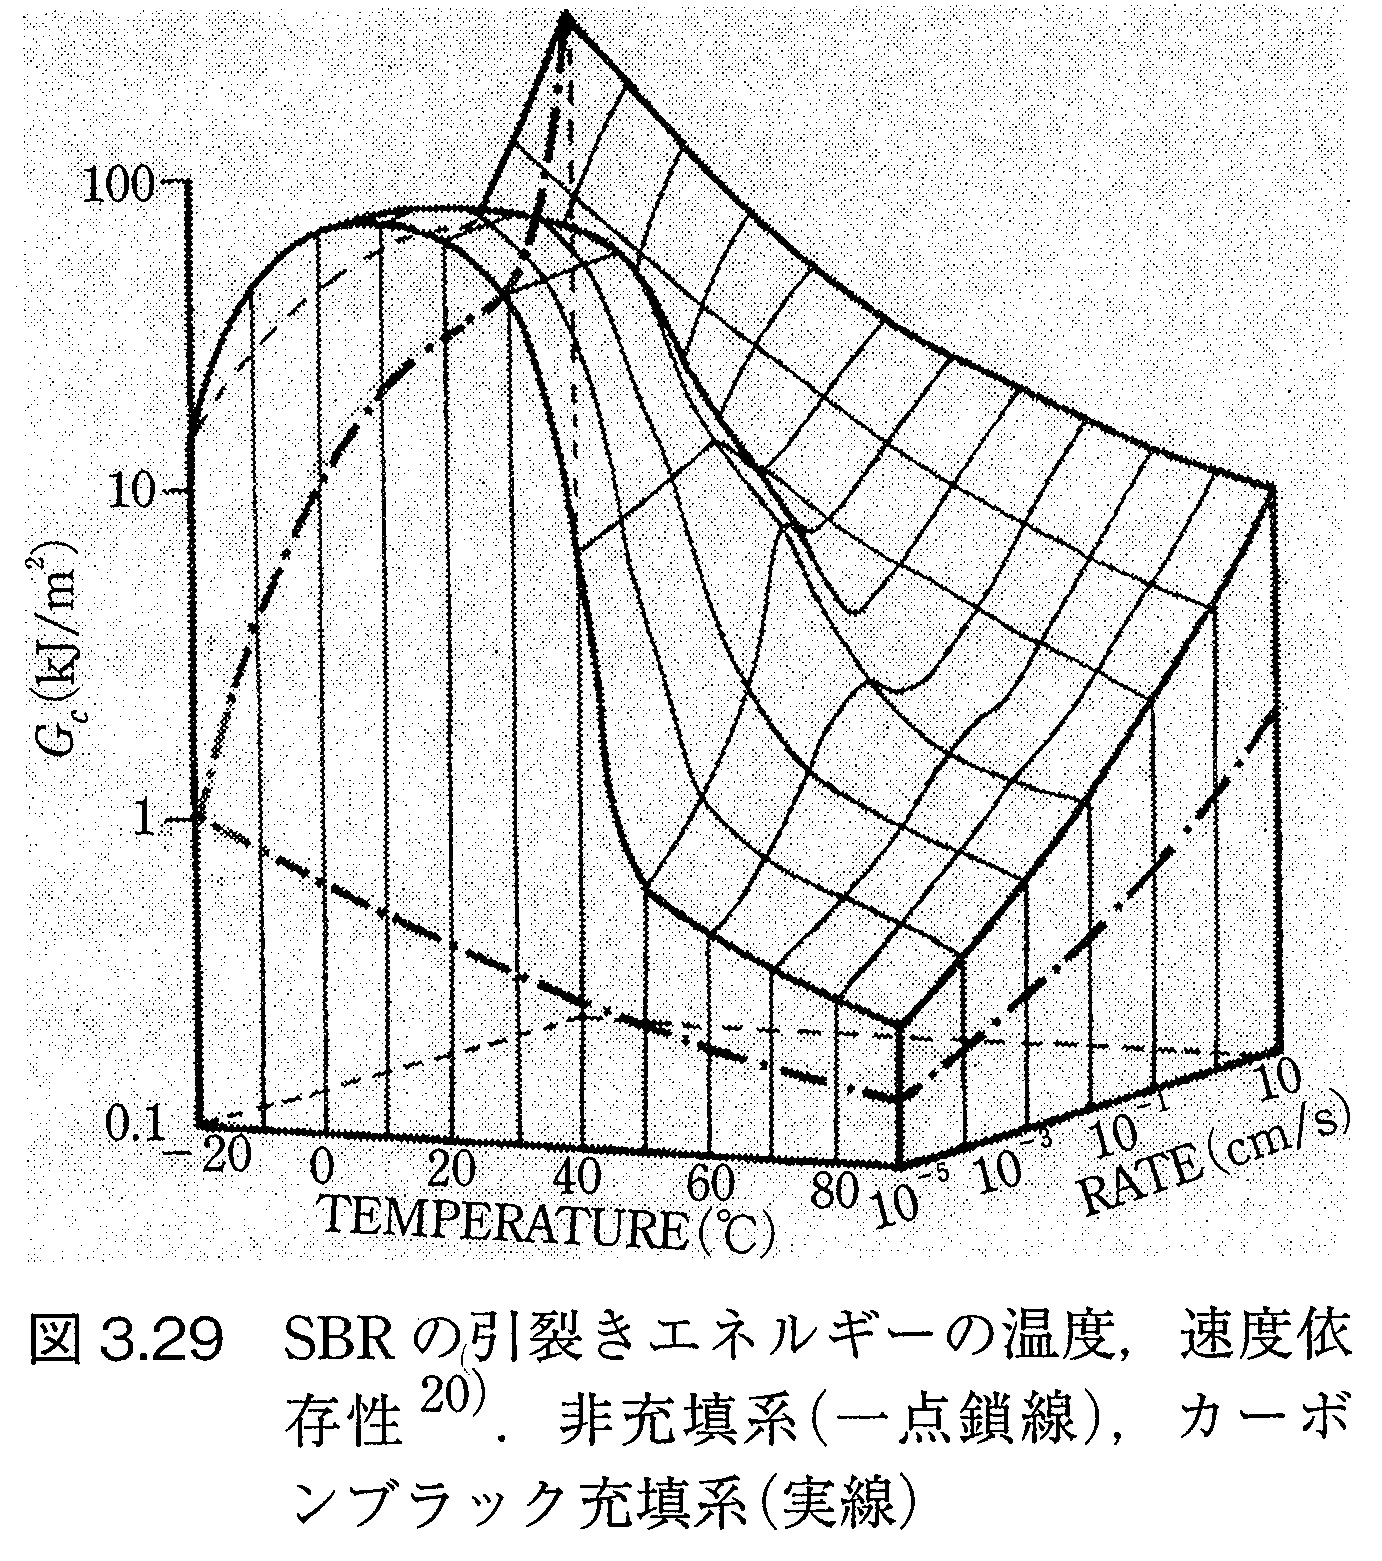
\includegraphics[width=0.8\textwidth]{./fig/break_TT.png}
\end{columns}
\end{frame}
%%%%%%%%%%%%%%%%%
\begin{frame}
\frametitle{天然ゴムとSBRとの違い(伸びきり効果の有無)}
\begin{columns}[totalwidth=1\textwidth]
\column{.48\textwidth}
伸長時の結晶化の有無で議論?
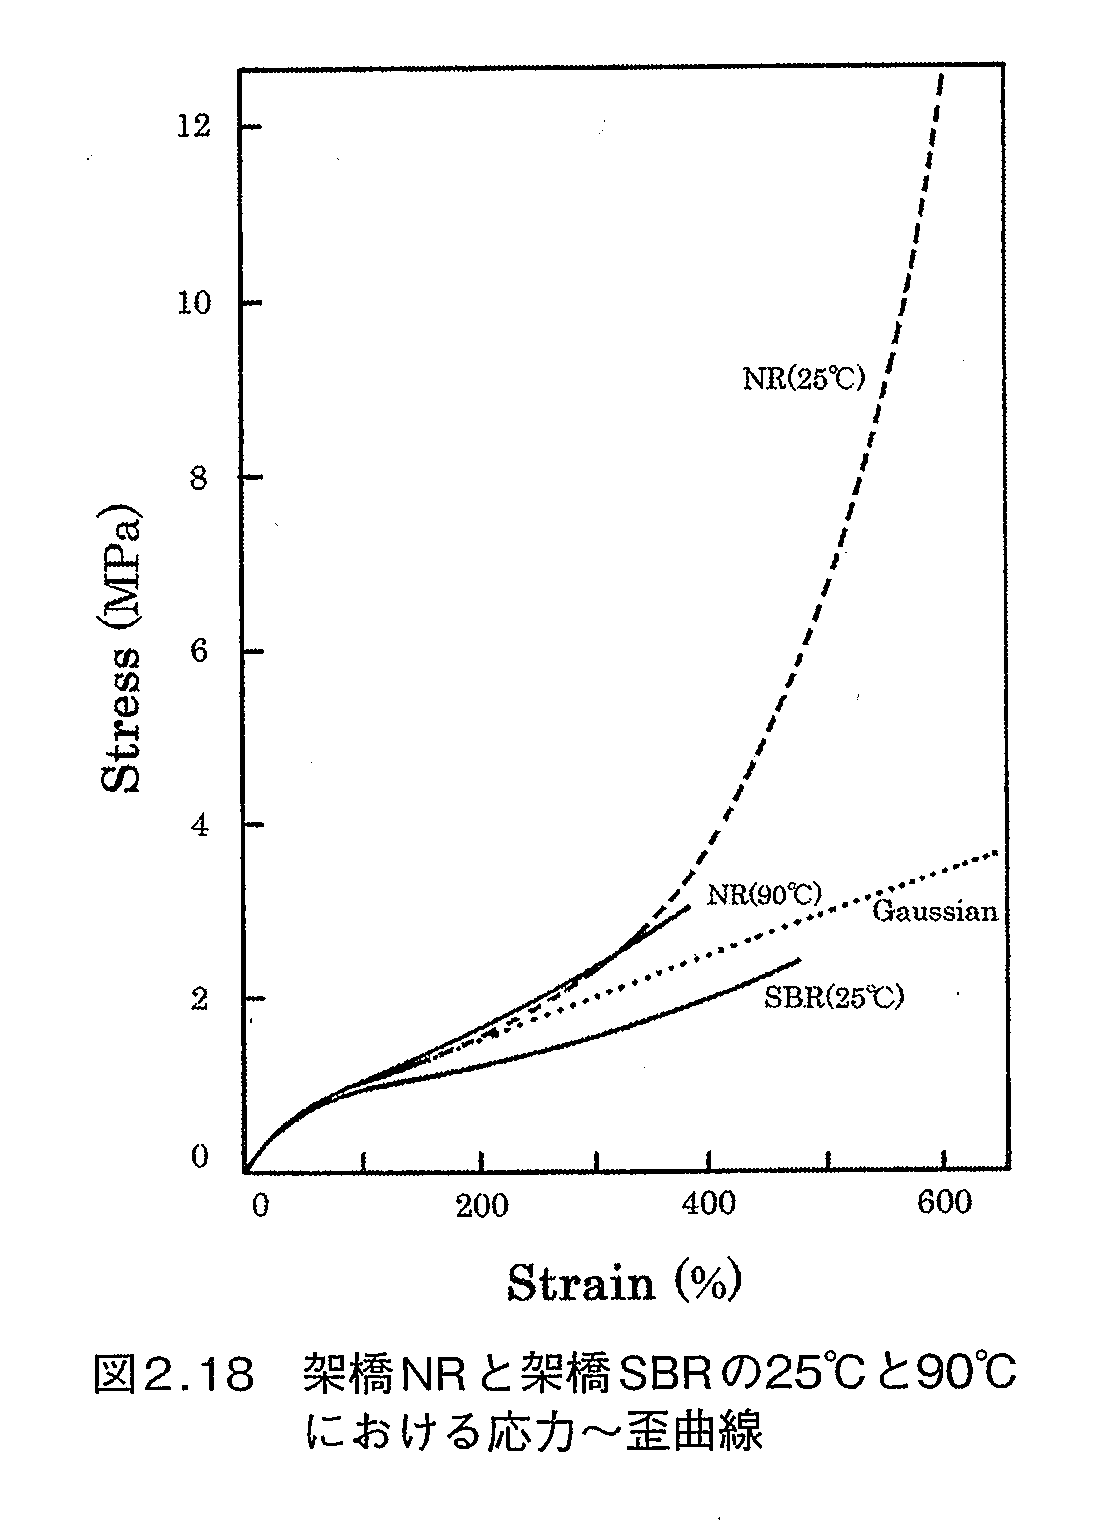
\includegraphics[width=0.7\textwidth]{./fig/NR_SBR.png}
\column{.48\textwidth}
低温であれば、SBRでも伸びきり効果が発現
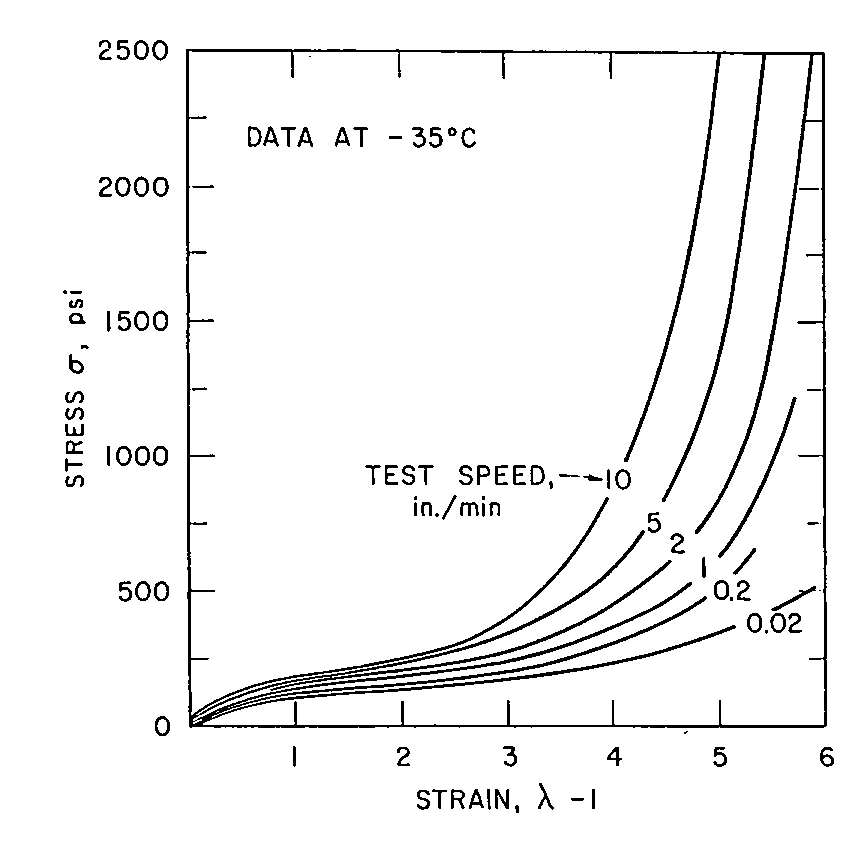
\includegraphics[width=0.9\textwidth]{./fig/SBR_lowTemp.png}
\end{columns}
\begin{alertblock}{時間温度換算則で考えてみれば?}
NR の適正な変形速度・温度と SBR のそれとの違い
\end{alertblock}
\end{frame}
%%%%%%%%%%%%%%%%%%%%%%%%%%
\begin{frame}
\frametitle{初期構造の作成}

\begin{enumerate}
\item
ストランドのセグメント数 $N$ と鎖のタイプを決める。
\item
ストランド長を自由鎖の二乗平均末端間距離とする。
$R=B\sqrt{C_{\infty}(N+1)}$
\item
8-Chainモデルでのユニットセルサイズ $a$ が決まる。
$a=\dfrac{2\sqrt{3}R}{3}$
\item
分岐数 m でユニットセル中のストランド数が決まる。
\item
設定したい密度 $\rho$ に対応する多重度 $M$ が決まる。
\end{enumerate}

分岐数 m=4 の例

\vspace{-1mm}
\renewcommand{\arraystretch}{1.5}
\begin{table}[htb]
 \centering
	\scriptsize
 \begin{tabular} {c c c c c c} \hline
 N		& R 		& a 		& Janction 	& Segments	& Denc. (Multi.) \\ \hline \hline
 34		& 7.48	& 8.64	& 4			& 138 		& 0.856 (M=4) \\ \hline
 55		& 9.46	& 10.93	& 4			& 222		& 0.850 (M=5) \\ \hline
\end{tabular}
\end{table}
\renewcommand{\arraystretch}{1.0}
\end{frame}
%%%%%%%%%%%%%%%%%%%%%%%%%%
\begin{frame}
\frametitle{ネットワークの分岐数の処理}
以下のようにノード番号を付与したネットワークを考えると、
\begin{center}
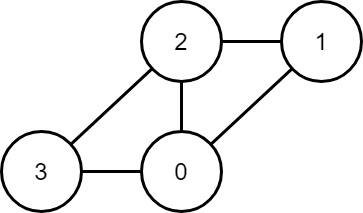
\includegraphics[width=4cm]{./fig/NW-4.png}
\end{center}
隣接行列、および、次数行列は、
\begin{align*}
A = \left( 
\begin{array}{cccc} 
0 & 1 & 1 & 1 \\ 
1 & 0 & 1 & 0 \\
1 & 1 & 0 & 1 \\
1 & 0 & 1 & 0 
\end{array} 
\right) 
,
D = \left( 
\begin{array}{cccc} 
3 & 0 & 0 & 0 \\ 
0 & 2 & 0 & 0 \\
0 & 0 & 3 & 0 \\
0 & 0 & 0 & 2 
\end{array} 
\right) 
\end{align*}
となる。
\end{frame}
%%%%%%%%%%%%%%%%%%%%%%%%%%
\begin{frame}
\frametitle{ラプラシアン行列}
\begin{columns}[totalwidth=1\textwidth]
\column{.48\textwidth}
ラプラシアン行列は、隣接行列$A$と次数行列$D$により以下のように定義される。
$$
L \equiv D-A
$$
4つのノードからなるネットワークの例であれば、
$$
L = \left( 
\begin{array}{cccc} 
 3 & -1 & -1 & -1 \\ 
-1 &  2 & -1 & 0 \\
-1 & -1 &  3 & -1 \\
-1 &  0 & -1 & 2 
\end{array} 
\right) 
$$
となり、非負の固有値を有する。
\column{.48\textwidth}
グラフが非連結であるとき、%ラプラシアン行列の成分を
連結した成分ごとにブロック対角化できるので、固有値 0 の重複数がグラフの連結成分ブロックの総数となる。
\begin{block}{「代数的連結性」}
「グラフが連結である場合、ラプラシアン行列の固有値 0 の重複数は 1」となる。\\
固有値を昇順にみた時、0 に次ぐ二番目の固有値がグラフの連結性の強さを示す指標となり、「代数的連結性」と呼ばれる。
\end{block}
\end{columns}
\end{frame}

%%%%%%%%%%%%%%%%%%%%%%%%%%%%%%%%%%%%%%%%%%
\begin{frame}
\frametitle{K4構造}
\begin{columns}[T, totalwidth=\linewidth]
\column{.32\linewidth}
\centering
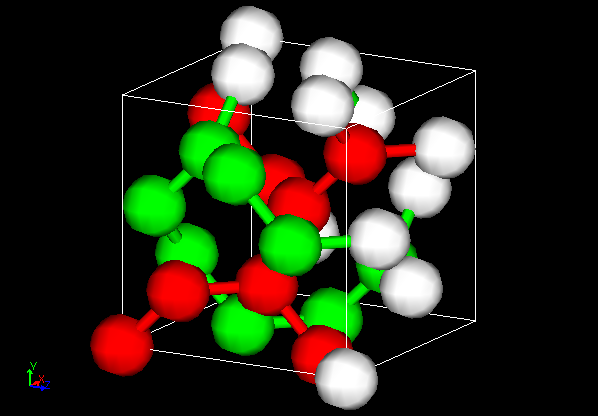
\includegraphics[width=\columnwidth]{./fig/K4_d.png}
\column{.32\linewidth}
\centering
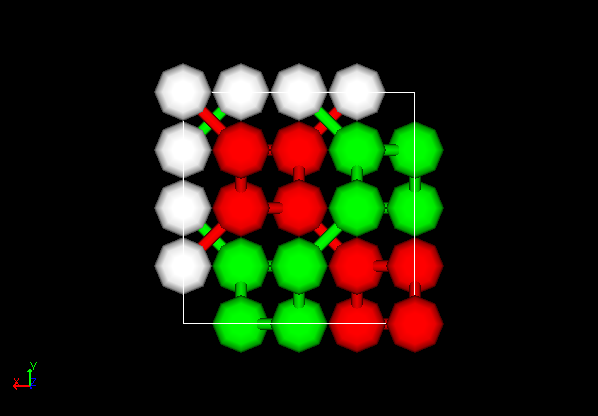
\includegraphics[width=\columnwidth]{./fig/K4_d_2.png}
\column{.32\linewidth}
\centering
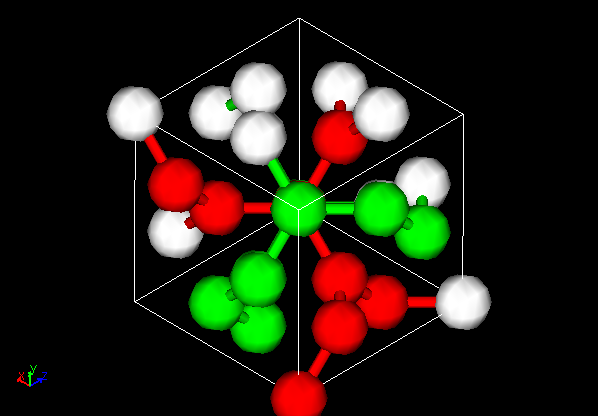
\includegraphics[width=\columnwidth]{./fig/K4_d_3.png}
\end{columns}
\end{frame}

\end{document}
